\documentclass{article}

%%Configurações padrão

\usepackage{indentfirst}
\usepackage[brazilian]{babel}
\usepackage[utf8]{inputenc}
\usepackage{graphicx}
\usepackage[a4paper]{geometry}
\pagestyle{headings}
\usepackage[round]{natbib}
\usepackage{caption}
\usepackage[nottoc]{tocbibind}
\usepackage{pdfpages}

%%Estilo PUC

\geometry{left=3cm}
\geometry{right=4cm}
%\geometry{top=2.5cm}
%\geometry{bottom=2.5cm}
%\geometry{textheight=24.7cm}
\geometry{textwidth=13.5cm}

\setlength{\topmargin}{1cm}
%\setlength{\headsep}{10pt}
%\renewcommand{\footskip}{2.5cm}
%\setlength{\headheight}{1cm}
%\setlength{\textwidth}{13.5cm}
%\setlength{\marginparsep}{3cm}
\renewcommand{\baselinestretch}{1.5}
%\setlength{\marginparwidth}{0pt}
%\setlength{\voffset}{-1in}
%\setlength{\hoffset}{-0.5cm}
\parindent 1cm

%%Depuração

%\usepackage{showframe}

\begin{document}

\thispagestyle{empty}
\phantom{----}
\vspace{4cm}
\begin{center}

\textbf{\LARGE{Discurso e Prática}}\\
\Large{A política fiscal brasileira entre 1997 e 1998}

\vspace{3cm}

\Large{Daniel Martins Coutinho}

\end{center}

\newpage
\thispagestyle{empty}

\begin{flushright}

%\includegraphics{../logopuc1}

\Large \textsf{Daniel Martins Coutinho}\\

\bigskip
\bigskip
\bigskip

\renewcommand{\baselinestretch}{1}

\Large \textsf{\textbf {Título da tese}}\\
\large \textsf{\textbf {subtítulo da tese}}\\

\bigskip
\smallskip

\large \textsf{\textbf {Informação da natureza acadêmica}}\\

\renewcommand{\baselinestretch}{1.5}

\bigskip
\smallskip

\large \textsf{Rogério L. F. Werneck}\\

\bigskip
\bigskip

\large \textsf{Rio de Janeiro}\\
\large \textsf{\today}\\

\end{flushright}

\newpage
\thispagestyle{empty}

\begin{center}

Agradeço a Rogério L. F. Werneck, meu orientador, pelas ideias, ajuda e suporte.
Ao MEC, pela Bolsa PET, sem o qual esta monografia não seria possível. 
Aos meus pais, pelo apoio.

\end{center}

\newpage

\setcounter{page}{1}
\tableofcontents

\newpage

\section{Introdução}

Em Junho de 1994, o povo brasileiro participou do capítulo final de uma saga: o fim da hiperinflação brasileira. Seis moedas depois, o Plano Real venceu a inflação crônica. Mas a saga não acabou ai.

A estabilidade da moeda depende de muitos fatores, dentre os quais uma condução firme da política monetária e uma política fiscal responsável. O Plano Real foi um passo importante para alcançar estas condições, mas não era suficiente para controlar a inflação no longo prazo. E um dos principais instrumentos usados pelo Plano para controlar a inflação, a âncora cambial, também estava intimamente relacionado com a política fiscal. Como observado por \citet[p. 332]{Werneck2014}, ``Para dar a sobrevida que acabou dando à manutenção do câmbio como âncora nominal, o governo teria de ter adotado política fiscal muito mais austera do que a que se permitiu manter". O país aprendeu a lição nos anos após a implementação do Real. %a lição? Não tá bom

O Brasil viveria, entre 1996 e 1998, anos tensos na frente econômica. Sofrendo com os efeitos adversos de duas crises internacionais, a asiática e russa, o governo e os brasileiros aprenderam o que os formuladores do plano real já sabiam: a necessidade de maiores reformas do que as realizadas em 1995. A tarefa mais importante era equilibrar as contas públicas. De fato, antes de 1996 - data na qual começa esta análise - algumas reformas tinham sido feitas. Mas as contas já voltavam a apresentar deficit em 1996.

O ano de 1996 foi relativamente calmo no cenário internacional, e será o ponto de partida para reconstruirmos os passos e tropeços da condução da política econômica em um país recém saído de uma hiperinflação. Cenário diferente foi o de 1997, com a crise asiática pegando o país de surpresa, um ano antes das eleições, com as polêmicas privatizações, o desequilíbrio das contas externas e outros problemas econômicos. A crise levaria o governo a agir em diversas frentes, inclusive no principal foco deste trabalho, a parte fiscal. O maior exemplo desta tentativa de reequilibrar as contas públicas foi o Pacote 51, apresentado no fim de 1997, com 51 medidas para reequilibrar as contas públicas.

O Pacote 51 também é o melhor exemplo de porque o país foi severamente afetado pela crise russa em 1998. Poucas propostas do pacote seriam, de fato, colocados em prática. E muitas delas seriam bastante alteradas no legislativo, mostrando que a condução da política econômica está, em última instância, sujeita ao jogo político. A crise russa levaria o país a abandonar a âncora cambial no início de 1999.  

Esta foi a situação da economia brasileira entre 1997 e 1998: graves desequilíbrios nas contas externas e nas contas do governo. Duas grandes crises externas que abalaram um país em recuperação de quase duas décadas de inflação alta. Um governo tentando navegar entre os limites da política e a política econômica responsável. É este o cenário explorado nas linhas abaixo.

\section{A economia brasileira entre 1996 e 1999}

A equipe econômica do governo Fernando Henrique - formada, em parte, por aqueles que criaram o Plano Real - sabia que a principal responsável pela inflação era o desequilíbrio fiscal do setor público. Assim, parecia natural que, uma vez no poder, o governo decidisse continuar a conter gastos e reduzir o deficit público.

Entretanto, não foi o que aconteceu: os anos de 1996 e 1997 tiveram deficit primário. A causa não foi a redução das receitas, mas sim devido a um aumento dos gastos. O tema é explorado com muito mais profundidade em \citet{Grossmann1998} e em \citet{Giambiagi2002}.
\smallskip

\begin{table}[h]
\begin{center}
\begin{tabular}[c]{|c|c|c|c|}
\hline
Ano & 1996 & 1997 & 1998\\ \hline
Deficit primário* & 0,09 & 0,97 & -0,02 \\ \hline
Governo Central* & -0,37 & 0,32 & -0,55\\ \hline
Estados e Municípios* & 0,54 & 0,72 & 0,18 \\ \hline
Empresas Estatais* & -0,08 & -0,07 & 0,35 \\ \hline
\multicolumn{4}{l}{*(-)=Superavit} \\
\multicolumn{4}{l}{Dados Obtidos de \citet{Giambiagi2002}} \\
\end{tabular}
\caption{Deficit Primário entre 1996 e 1998 como \% do PIB}
\end{center}
\end{table}

Vemos na tabela 1 que, apesar de o cenário não ser bom em 1996, ele é melhor do que o ano de 1997 - o mesmo ano da crise da Ásia e do pacote do governo que pretendia reduzir os gastos. Poderíamos argumentar que 1997 não seria afetado pelo Pacote porque ele foi concebido no fim do ano, e muitas medidas só foram aprovadas no ano seguinte. %Ver a data do acordo e se o Giambiagi fala isso

São muitas as hipóteses por trás da deterioração das contas públicas no período: \citet{Werneck2014} sugere que o fim da inflação é um responsável pela deterioração do quadro fiscal. \citet{Giambiagi2002} oferece outra hipótese: para ele, os gastos do governo aumentaram, especialmente em relação ao aumento dos gastos com pessoal. Uma discussão detalhada do tema pode ser encontrada em \citet{Grossmann1998}.

Independente do responsável pelo aumento do déficit primário no período, a equipe econômica realizaria diversos cortes nos gastos com pessoal no período estudado, como pode ser observado na Tabela \ref{tab:DepesaPessoal}.

\begin{table}[h]
\begin{center}
\begin{tabular}[c]{|c|c|c|c|}
\hline
Ano & 1996 & 1997 & 1998\\ \hline
Despesa total com pessoal & 5,25 & 4,76 & 5,02 \\ \hline
Ativos & 2,66 & 2,35 & 2,37\\ \hline
Inativos & 2,33 & 2,19 & 2,43 \\ \hline
Empresas Estatais* & -0,08 & -0,07 & 0,35 \\ \hline
\multicolumn{4}{l}{*(-)=Superavit} \\
\multicolumn{4}{l}{Dados Obtidos de \citet{Giambiagi2002}} \\
\end{tabular}
\caption{Despesa com pessoal como \% do PIB} \label{tab:DepesaPessoal} %colocar variação entre 1996 e 1998?
\end{center}
\end{table}

Como se vê, a despesa com pessoal como porcentagem do PIB não aumentou. Pelo contrário, entre 1996 e 1998, o gasto como \% do PIB caiu. Isso se deve, principalmente, a redução com gastos no pessoal na ativa. Nas seções a seguir, veremos que o governo tomou medidas para reduzir a quantidade de servidores durante o período estudado.

É importante analisar, também, a evolução do resultado nominal, que leva em conta os gastos do governo com a dívida. Com as diversas crises internacionais e com o câmbio fixo, o Banco Central debelou ataques contra o Real usando a taxa de juros, afetando as contas do governo. %que engloba...

\begin{table}[h]
\begin{center}
\begin{tabular}[c]{|c|c|c|c|}
\hline
\textbf{Ano} & \textbf{1996} & \textbf{1997} & \textbf{1998}\\ \hline
Deficit primário* &  &  &  \\ \hline
Governo Central* &  &  & \\ \hline
Estados e Municípios* &  &  &  \\ \hline
Empresas Estatais* &  &  &  \\ \hline
\multicolumn{4}{l}{Dados Obtidos de \citet{Giambiagi2002}} \\
\end{tabular}
\caption{Deficit Operacional entre como \% do PIB}
\end{center}
\end{table}

São esses os números do período. Como a situação se desenvolveu é o tema da análise da próxima seção. 

%A situação da economia, tanto brasileira como mundial, que contribuíram para o surgimento de problemas e desconfianças em relação a condução da política econômica. O Plano Real sofreu um primeiro ``teste'' internacional com a crise do México, em Dezembro de 1994. Em 1997, seria a vez da Ásia entrar em crise, afetando mais uma vez o Brasil. E, em 1998, a Rússia sofreria uma crise. Todos esses países tinham um câmbio fixo, ou o câmbio flutuava dentro de uma banda - como era o caso do Brasil. O México e diversos países da Ásia sofriam com déficits na Balança de Pagamentos; a Rússia tinha deficit fiscal. E o Brasil tinha tanto deficit na Balança de Pagamentos quanto deficit fiscal, transformando o país em alvo de especulações em cada uma dessas crises. 

%Se o cenário internacional do período era conturbado, o Brasil não se encontrava em situação melhor. Um fator comum afetaria todos os anos da análise: a emenda da reeleição e a campanha de Fernando Henrique Cardoso para ser reeleito. Há poucas dúvidas de que, para aprovar a emenda, o presidente teria que ser generoso com a base aliada, governadores e prefeitos, já apontado em \citet{Werneck2014}. E ainda, ele não poderia implementar medidas impopulares - mas necessárias -  no ano das eleições, sob risco de perder as eleições. 

%Outros fatores além da política afetariam o país: a falência de vários bancos em 1996, seguido de acusações de corrupção por parte dos mesmos. As privatizações, que enfrentariam imensa resistência política.  Além disso, alguns membros da equipe econômica do governo não concordavam com a âncora cambial, gerando divisões que não afetariam todo o processo decisório da equipe, como observado em \citet{Werneck2014}.  

\section{A política econômica brasileira entre 1996 e 1999}

Os jornais são uma fonte valiosa de informações sobre a economia e a política fiscal brasileira. Entrevistas e declarações de diversos economistas membros da equipe econômica da época podem ser encontradas nos acervos dos jornais, assim como estatísticas e notícias que nos ajudam a reconstruir os acontecimentos dos anos de 1996 à 1998. 

\subsection*{1996}
\addcontentsline{toc}{subsection}{1996}

Mesmo sem sofrer com uma crise econômica internacional, o ano de 1996 foi conturbado. O cenário político assistiria as tentativas de aprovação da emenda da reeleição, que sofreu imensa resistência do congresso, além da prisão de diversos funcionários de bancos brasileiros, que em última instância levaria a intervenção do Banco Central nestes bancos e gastos do governo para evitar uma crise no sistema financeiro. Os problemas econômicos também foram manchetes, e o descontrole fiscal já era claro.

Acima de tudo, o ano de 1996 assistiria um governo ``bipolar": às vezes, o governo defendia veementemente as reformas administrativas, para cortar gastos e reduzir os desequilíbrios nas contas públicas. Outras vezes, o governo se via obrigado a abrir o cofre e trocar favores. A Folha de São Paulo trazia a seguinte manchete no dia 21 de março: ``FHC troca favores troca favores pelo fim da CPI".  Os favores incluíam assumir uma dívida de 3 bilhões de reais do prefeito de São Paulo e a liberação de verbas para a Roseana Sarney, governadora do Maranhão, cujo o pai, José Sarney, era a favor da CPI. %trocar este último trecho sobre o sarney

A CPI pretendia investigar os bancos que quebraram com o fim da inflação, as alegações que políticos estariam envolvidos - inclusive o próprio presidente da República - e o resgate dos mesmos. Os bancos foram um problema para a equipe econômica em 1996. Durante a hiperinflação brasileira, os bancos criaram mecanismos que permitiam com que eles ganhassem dinheiro com a inflação. O fim da hiperinflação acabou com essa fonte de receitas e levou várias instituições a falência. Os Banco Central criou o Programa de Estímulo à Reestruturação e ao Fortalecimento do Sistema Financeiro Nacional, para resgatar os bancos privados que faliram e evitar uma crise no sistema financeiro. Muitos bancos foram acusados de corrupção, e funcionários de alguns deles foram presos. O caso mais notável é o do banco Nacional, cuja a prisão do contador e de um ex-diretor seriam manchetes do O Globo de 16 de março e da Folha de São Paulo do mesmo dia.

Não seriam apenas os bancos privados que sofreriam com problemas financeiros. A Folha de São Paulo de 21 de março trazia na capa, a noticia de que o Banco do Brasil teve prejuízo e que o socorro ao banco aumentaria a dívida pública em pelo menos R\$2,32 bilhões. A notícia também deixava claro que pelo menos os jornais entendiam a necessidade do equilíbrio das contas públicas: ``O descontrole das contas públicas é a principal ameaça ao Real" dizia um parágrafo da notícia sobre o socorro ao Banco do Brasil. E continuava ``O Tesouro Nacional já acumula um rombo de R\$3,6 bilhões em 1996". 

Evidentemente, o governo era obrigado a negociar as reformas para reduzir gastos, e para isso acabava trocando favores. O caso mais emblemático foi o da reforma da previdência, uma das reformas que faria o governo economizar dinheiro. Graças a troca de favores a câmara aprovou a reforma. A Folha de São Paulo do dia 22 de março relatava que ``Para conseguir as vitórias, FHC ofereceu cargos e obras a Estados e assumiu as dividas". Não seria o bastante e mais favores seriam necessários: no dia 16 de Maio, a Folha de São Paulo informava que o governo tinha autorizado, entre outras coisas, a transferência de R\$892 milhões para uma empreiteira para garantir votos para a aprovação da reforma da Previdência. Mas nem mesmo as trocas de favores seriam capazes de garantir totalmente a reforma da previdência. Três pontos considerados essenciais pelo governo foram derrubados, como relata a Folha de São Paulo do dia 23 de Maio.

Em meio as derrotas, favores e negociações, a dívida pública aumentou. ``FHC faz o maior déficit dos 90", informava a Folha de São Paulo do dia 24 de Fevereiro. ``Dívida federal bate recorde histórico" era a manchete do mesmo jornal no dia 11 de Abril. As causas parecem ser, acima de tudo, os gastos com pessoal: o subtítulo da manchete de fevereiro da Folha já citado era ``O rombo, gerado por aumento das despesas com juros da divida interna e com pessoal, equivale a 4,95\% do PIB". Explicação parecida dava O Globo do dia primeiro de Abril, que informava na capa que ``Governo gastou mais com pessoal do que arrecadou" e ainda informava que ``Em janeiro, despesa com salários e encargos chegou a 101\% da receita". O deficit já era maior em abril do que em fevereiro, chegando a 6,3\% do PIB.

A reportagem do O Globo do dia primeiro de Abril trazia algumas informações importantes. O desequilíbrio fiscal já preocupava os investidores estrangeiros. O diretor da Bear Stearns garantiu que ``os investidores estrangeiros não estão batendo em retirada, mas estão mais cautelosos e reduziram o volume de negócios no país". Na mesma reportagem, economistas entrevistados pelo jornal afirmavam que ``o Governo têm poucas chances de controlar o déficit esse ano". O principal motivo apontado foi as eleições municipais de 1996, já que a principal sugestão para ajustar as contas públicas era ``conter os reajustes do salário mínimo e do funcionalismo". Também foi observado que ``o governo federal não é o único responsável pelo deficit. A situação das finanças dos estados e municípios também é preocupante".  

O mesmo aumento nos gastos com pessoal é observado em \citet{Giambiagi2002}. O autor calcula que, em média, o crescimento da quantidade de benefícios entre 1994 e 1998 foi 4,2\% a.a. O crescimento das aposentadorias no mesmo período foi, em média, 4,1\% a.a. Giambiagi também aponta que 44 \% dos gastos com pessoal em 1995 era com inativos. Não surpreende que o governo tenha lutado tão arduamente para aprovar as reformas na Previdência.   

O deficit acontecia apesar de aumentos na arrecadação. A CPMF foi aprovada em Julho e foi alvo de negociações. O governo queria que o imposto tivesse alíquota de 0,25\% e durasse dois anos, mas só conseguiu 0,20\% e duração de um ano, segundo a Folha de São Paulo de 11 de Julho. Os recursos obtidos com o imposto foram destinados à saúde. E, apesar de defender um ajuste fiscal, o ministro da fazenda, Pedro Malan, e do planejamento, Antonio Kandir, eram contra, assim como o presidente do Banco Central na época, Gustavo Loyola. Informava a Folha de São Paulo que a equipe econômica ``avalia que o novo imposto do cheque vai aumentar as taxas de juros e pressionar os custos das empresas. Isso pode resultar em reajuste de preços, pondo em risco o Plano Real."

Por que aumentar impostos quando, claramente, a equipe econômica era contra? Por que não realizar cortes, como os que seriam feitos mais tarde, depois da Crise da Ásia? Por que não insistir nas reformas constitucionais?

Como para qualquer questão muito complexa, é difícil definir uma causa única. Vale reproduzir um dos argumentos, o de \citet[p. 341]{Werneck2014}:

\begin{quote}
``Ironicamente, parte da dificuldade de fazer avançar o programa de reformas advinha do próprio sucesso do programa de estabilização. Com o crescente otimismo acerca da evolução do quadro inflacionário, havia desaparecido boa parte do senso de urgência que emanava da apreensão com o regime de alta inflação. E não era só no Congresso que se podia detectar perda de convicção sobre a real necessidade das reformas. No próprio Executivo, surgiram duvidas sobre o acerto da insistência num programa de reformas constitucionais que exigia prolongada manutenção de desgastante maioria de 60\% nas duas casas do Congresso"
\end{quote} 

A reação do executivo também tem uma outra razão política: a emenda da reeleição. A constituição de 88 não autorizava a reeleição. Fernando Henrique Cardoso tentou aprovar a emenda da reeleição, que sofreu grande resistência. Precisando de 308 votos, o levantamento feito pelo O Globo no dia 8 de setembro dizia que 116 deputados aprovariam a emenda. Uma pesquisa feita mais tarde no mesmo ano pelo governo dizia que a emenda só teria 263 votos garantidos, informava O Globo de 14 de novembro.

Políticos com grande influência - incluindo aliados do governo - eram contra a emenda. Uma pesquisa encomendada pelo governo que apontava a vitória de FHC caso houvesse reeleição trouxe problemas para o governo, como informava O Globo de 30 de Agosto. ``Itamar, Sarney, Lula e Maluf reagem à pesquisa do Planalto e se manisfestam contra reeleição", era o subtítulo da noticia do O Globo.

Neste cenário, não surpreende que o ajuste fiscal não tenha sido uma prioridade, especialmente o corte de gastos, sempre impopular entre os congressistas e entre os possíveis eleitores. Por exemplo, Maluf - aliado do governo - disse, em declaração para O Globo de 30 de Agosto que ``Os tucanos estão perdendo em todas as cidades importantes". Não surpreende que o presidente tenha evitado tomar decisões impopulares.

Porém, a impopularidade das reformas não impediria que o governo agisse, especialmente se não precisasse passar pela aprovação do congresso. E, via Medida Provisória, o governo poderia agir e depois obter a aprovação do congresso. E assim foi feito. Anunciava O Globo do dia 12 de Outubro, na primeira página do caderno Economia: ``O pacote de medidas baixado pelo Governo ontem tem um objetivo claro: reduzir o déficit do setor público, o principal problema do Plano Real". O pacote agia em duas frentes, tanto cortando despesa - com destaque para a extinção de cem mil cargos públicos e para as reformas que visavam desincentivar a aposentadoria precoce - quanto aumentando a receita. A economia estimada era de R\$6,5 bilhões. A medida não afetou Estados e municípios, a única parte do governo que apresentou deficit primário em 1996.

%Não faltavam explicações de por que o governo estava agindo via MP, e O Globo relatava que ``[a] aprovação da reforma administrativa [é] mais difícil de ser negociada no atual contexto de discussão da reeleição do presidente Fernando Henrique Cardoso". Haviam também muitas explicações em relação ao aumento do déficit, e O Globo dedicou um parágrafo inteiro para explicar a tese de que o próprio fim da inflação teria aumentado o déficit.

Deve-se observar que a própria equipe econômica reconhecia a limitação das reformas que eram possíveis via Medida Provisória. Na coluna \textit{Panorama Econômico} do dia 12 de Outubro, Pedro Malan dizia que ``Não é que sem as reformas [constitucionais] a situação vai mudar radicalmente. Só que com elas poderia ir muito melhor. Os frutos serão maiores quanto mais rapidamente avançarmos na reforma da Constituição". 

A constituição de 1988, desde antes de sua promulgação, foi alvo de fortes criticas de economistas. Um dos mais importantes economistas brasileiros, Mário Henrique Simonsen, escreveu dois artigos para jornais criticando a constituição. Em coluna no O Globo de 19 de Outubro de 1986, Simonsen escreveu que ela continha ``um verdadeiro tratado de antieconomia." O economista afirmou que limitar a participação de empresas estrangeiras na economia é uma receita para limitar o desenvolvimento. Outra crítica diz respeito a quantidade de direitos garantidos na constituição, sem que se leve em conta o fato de que alguém terá de pagar por eles.

Gustavo Franco, um dos idealizadores do Plano Real e mais tarde presidente do Banco Central, analisando a hiperinflação brasileira quase 10 anos depois do Plano, disse que:

\begin{quote}
``Não é outra a essência da crise fiscal brasileira: desejos, que se tornaram direitos, às vezes extravasando o terreno orçamentário e inscrevendo-se mesmo na Constituição, maiores que as possibilidades fornecidas pela tributação.[...] E assim, o quanto mais se pretendia resolver as mazelas do país “por decreto”, no Orçamento Geral da União, ou mesmo na Constituição, fixando níveis irreais de despesa, mais alta se tornava a taxa de inflação necessária para trazer a despesa pública \textit{ex post} para níveis consistentes com a realidade da receita pública" \citep{Francoxxxx}
\end{quote}

Assim, não surpreende porque o ministro da fazenda pleiteava reformas na constituição: ao garantir direitos demais, a constituição pressionava as contas públicas. Equilibrar as contas públicas era uma tarefa extremamente complicada sem mudanças na constituição. 

E, na mesma entrevista da declaração do ministro Pedro Malan, o ministro do Planejamento, Antônio Kandir, dizia que o crescimento do PIB ``depende de reforma constitucional que viabilizará a formação de poupança interna", ecoando as ideias que Mário Henrique Simonsen defendeu 10 anos antes.  

Enquanto em 1996 o governo encontrou resistência nas reformas, dificuldades para estabilizar as contas públicas e desafios políticos, 1997 prometia ser um ano de ajustes. Ou pelo menos essa era a promessa do Orçamento de 1997 entregue pelo governo, informava O Globo de 31 de Agosto. ``Proposta enviada ao Congresso prevê um ano de arrocho nas contas públicas" era o subtítulo da matéria, que indicava que o governo pretendia reduzir ainda mais os gastos com pessoal. As contas apresentadas pelo O Globo sugeriam um superavit de aproximadamente R\$3 bilhões.

\begin{table}[h]
\begin{center}
\begin{tabular}[c]{|c c|}
\multicolumn{2}{c}{\large\textbf{Os número do orçamento de 97}}\\ \hline \normalsize
 Receitas & R\$ 177,1 bilhões   \\ \hline
 Despesas & R\$ 174,8 bilhões  \\ \hline
 Pessoal &  R\$ 45 bilhões  \\ \hline
 Previdência & R\$ 46,3 bilhões   \\ \hline
 Investimentos & R\$ 7,7 bilhões  \\ \hline
 Juros &  R\$25,2 bilhões \\ \hline
 Saúde & R\$ 13,8 bilhões \\ \hline
 Ensino Básico &  R\$ 1,9 bilhões \\ \hline
 Seguro Desemprego & R\$ 5,2 bilhões  \\ \hline
 Reforma Agrária &  R\$901,4 milhões \\ \hline
\multicolumn{2}{l}{Fonte: Ministério do Planejamento} \\
\end{tabular}
\caption{Quadro sobre o orçamento de 1997, reprodução do O Globo de 31 de Agosto,p. 12 (em valores da época)}
\end{center}
\end{table}

Em 1996 o governo tentou encontrar um equilíbrio entre o jogo político e a política econômica, evitando decisões problemáticas, tendo em vista o cenário conturbado no congresso. A tentativa de agradar todos os lados cobraria o seu preço em 1997.  

\subsection*{1997}
\addcontentsline{toc}{subsection}{1997}

O ano de 1997 começaria com uma boa notícia para o presidente Fernando Henrique: a aprovação da emenda da reeleição. No dia 29 de Janeiro, o Globo noticiava a vitória da emenda, que ocorreu em um cenário complicado, com membros de partidos da base aliada se opondo a ela. Assim, já em 1997, o presidente poderia começar a fazer campanha.

No dia dois de Julho, O Globo trazia a seguinte manchete``FH: Sem reforma faltarão recursos para governar". A reportagem, que tem como título ``Presidente dá ultimato ao congresso" e informa, no subtítulo que ``FH diz que, sem elas [as reformas], não terá como governar". Mais significativo é que, acima do título, o jornal informava que FH estava ``Falando como candidato", e na própria notícia era dito que ``Fernando Henrique diz que não se importa com acusação de campanha".

É interessante observar, entretanto, que na notícia do dia dois de Julho, o próprio presidente admitia que ``o Governo enfrenta dificuldades internas em relação a reforma tributária" e que não havia condições de retirar mais recursos da união. É bem provável que a principal dificuldade do governo fosse cortar gastos, e principalmente, cortar os gastos dos estados e municípios.\footnote{É importante observar que, além de realizar transferências para estados e municípios, o governo sempre renegociava a dívida destes e, não raramente, salvava estados em dificuldade. Isso só mudaria com os acordos de refinanciamento e a Lei de Responsabilidade fiscal. Para mais detalhes, ver \citet{Giambiagi2002}}

A defesa da reforma tributária - a ponto do presidente falar em um ultimato - se deve a uma derrota anterior: a da reforma administrativa, que visava reduzir os gastos do governo. Em 8 de junho, O Globo noticiava que o líder da câmara, Luís Eduardo Magalhães, aliado de FHC, achava que a reforma administrativa estava perdida, pelo menos nos principais pontos: ``o fim da estabilidade e estabelecimento do teto salarial para funcionários públicos". Aliados do governo culpavam o próprio governo pelas ``sucessivas derrotas em votações da reforma administrativa". Na mesma página, o jornal também informava que o maior problema não era a oposição, mas os aliados do governo. 

Apesar de toda a retórica do presidente em realizar reformas para reequilibrar as contas públicas, nem mesmo ele deixaria de usar instrumentos antigos na política brasileira. Para garantir a prorrogação do Fundo de Estabilização Fiscal (FEF), que foi essencial para o sucesso do Plano Real, o presidente negociou empréstimos para os prefeitos que eram contra a prorrogação da FEF, informava O Globo de 15 de Julho de 1997. A reportagem evidenciava esta contradição, já que no mesmo evento Fernando Henrique Cardoso dizia que não permitiria ``a volta a 'gastança' em véspera de eleição". As ambiguidades de 1996 continuavam existindo. Dois dias depois, O Globo noticiava que o governo tinha conseguido aprovar a FEF, que desvinculava R\$70 bilhões. 

A aprovação veio em boa hora: a crise asiática, que começou em Julho, afetou o país. Um dia antes da aprovação do Fundo de Estabilização Fiscal, a manchete da Folha de São Paulo anunciava o desastre: ``Efeito Ásia derruba as Bolsas". A queda da Bolsa de São Paulo era a maior desde 1995, e se a situação externa não era boa, o governo sofreu com o fogo amigo: o ministro das Comunicações, Sérgio Motta, critcaria Gustavo Franco, ainda diretor do Banco Central, o que derrubaria ainda mais a bolsa. 

A crítica de Sérgio Motta se deve a uma discussão antiga em relação a da âncora cambial. Como parte do Plano Real, a moeda nova era atrelada ao Dólar. A crise na Ásia começou justamente com um ataque ao câmbio na Tailândia, que também adotava uma âncora com o Dólar. O debate tinha começado ainda no início do primeiro mandato de FHC, como observa \cite[p. 332]{Werneck2014}. Reavivar o tema na esteira de uma crise era uma receita para problemas. E, no dia 17 de Julho, o governo já tentava consertar o estrago: O Globo informava que Sérgio Motta tinha sido proibido pelo presidente de comentar ``qualquer assunto na área econômica".

Sérgio Motta ainda sofreria mais uma derrota, noticiada pelo Globo no mesmo dia. O dinheiro arrecadado com as privatizações foi objeto de controvérsia, com o ministro das Comunicações querendo que pelo menos parte do dinheiro fosse investido ou usado em projetos na área social; a equipe econômica era a favor de usar os recursos para abater a dívida. FHC bateu o martelo e destinou todo o dinheiro para abater a dívida, pondo um ``fim a uma discussão que vinha se arrastando há meses dentro do Governo", como observava o jornal. O governo parecia, afinal, ter notado que era hora de agir.

Isso não significa que era uma opinião comum que a crise na Ásia fosse atingir o Brasil. Pelo contrário. No dia 15 de Julho, no O Globo, o caderno de economia trazia uma reportagem intitulada ``Analistas rejeitam possibilidade de que a crise nos `tigres' atinja também o Brasil". No dia seguinte, Armínio Fraga deu uma entrevista ao Globo. Quando perguntado se o Brasil poderia sofrer um contágio da crise da Ásia, ele responderia que ``[...] para o Brasil, a situação não é preocupante"  

Os maiores alertas partiram de um dos formuladores do Plano Real. Winston Fritsch, já afastado do governo na época, alertava no O Globo de 20 de Julho que ``embora a situação brasileira não encontre paralelo na tailandesa, se o país continuar deitado em berço esplêndido irá se transformar na Tailândia." 

Mas, em um primeiro momento, não parecia haver motivos para se preocupar. No dia 17 de Julho, um dia após a manchete na Folha de São Paulo sobre a queda na bolsa, a primeira página do O Globo anunciava a alta das bolsas brasileiras com o título ``Bolsas espantam o fantasma da crise".    

Na verdade, o governo ainda teve mais uma boa notícia: o déficit do setor público caiu de 5,53\% do PIB para 4,94\% segundo noticiado pelo O Globo de 26 de Agosto. Isso não se deve, exclusivamente, ao resultado do nível federal. ``Estados e municípios também deram sua contribuição" informava a reportagem do O Globo. Parecia, afinal, que as medidas do governo tinha tido efeito. 

É necessário um parentese: apesar de tratarmos centralmente da política fiscal, a política monetária merece algumas considerações. Sem o necessário ajuste fiscal, caberia a política monetária impedir o retorno da inflação. Na posse como presidente do Banco Central, Gustavo Franco anunciaria que ``As âncoras são para sempre". O subtítulo da matéria do O Globo o dia 21 de Agosto sobre a posse deixava claro que ``não há planos para mudar política cambial". E a reportagem ainda reproduzia o seguinte trecho do discurso do novo presidente do BC: ``O Banco Central não fabricará dinheiro para deprimir os juros quando o Estado os pressiona para cima tomando dinheiro emprestado, pois assim estaríamos indiretamente e, hipocritamente, financiamento o déficit público com a emissão de moeda." %precisa desse parágrafo?

A crise asiática continuaria afetando as bolsas do mundo, sendo tema de reportagens no dia 29 e 30 de agosto nos jornais O Globo e Folha de São Paulo. Setembro seria relativamente mais calmo: nenhuma manchete da Folha nem do O Globo seria dedicada a crise internacional e os efeitos dela no Brasil. E também não haveria novos anúncios de reformas do governo, que ainda acertava alguns detalhes da reeleição.

E o início de Outubro também seria calmo, com as manchetes falando mais sobre a visita do Papa e de Bill Clinton, presidente dos Estados Unidos na época, do que da crise na Ásia e seus efeitos no Brasil. Mas no dia 24 de Outubro, o cenário mudou. Hong Kong aumentou os juros e virou capa do O Globo e da Folha. As bolsas despencaram. No dia seguinte O Globo trazia como manchete a declaração de Pedro Malan de que a ``crise das bolsas não afeta o Brasil". Na reportagem, o ministro ressaltava as diferenças entre os países asiáticos e o Brasil. As diferenças eram mais quantitativas: o tamanho do déficit externo e como ele era financiado foi ressaltado pelo ministro. Não que  Malan fosse o único a afirmar que a nossa situação era diferente da Ásia. Mas, pelo menos, ele reconhecia que ``o espaço para erro na condução da política econômica atualmente é muito menor". E ainda, o ministro informava que não iria permitir com que o Brasil tivesse um déficit em transações correntes iguais o da Tailândia.        
 
Era bom saber que o ministro da Fazenda estava alerta. Pior era saber que a diferença entre o nosso déficit em transações correntes e o da Malásia era de 4\% . Miriam Leitão, em sua coluna do dia 25 de Outubro - mesmo dia da entrevista de Pedro Malan - dizia exatamente isso. Ela também apontava que a crise tinha atingido Hong Kong, onde o déficit na conta corrente era muito menor do que no Brasil. Por que ainda não sido atingido pela crise? A resposta de Miriam Leitão era que ``o mais relevante para os investidores é a percepção que tenham da convicção e coerência da política econômica". A jornalista seguia apontando os erros dos países da Ásia, e apontava que, em contraste, o país caminhava bem: o país estava, pelo menos, tentando reduzir os déficits públicos e externos, tentando realizar reformas. Segundo a jornalista, este era o nosso trunfo. 

Mas o mercado não parecia tão otimista, e voltou a derrubar as bolsas no mundo, especialmente a Bovespa. A capa do O Globo de 28 de Outubro era explícita: ``Pânico nas bolsas do mundo". Wall Street caiu mais de 7\% e a Bolsa de São Paulo, quase 15\%, a maior queda no mundo. Alguns títulos da dívida externa brasileira eram negociados a 68\% do valor de face, em contraste com os 82\% da sexta anterior, refletindo a desconfiança em relação ao país. O presidente do Banco Central, Gustavo Franco, declarou que ``a queda da Bovespa é um fenômeno `restrito a bolsa'".

No dia seguinte, o fenômeno não seria mais restrito a bolsa, e o Banco Central teria de agir para  conter ``movimento especulativo no câmbio", como informava a capa do O Globo. Sete leilões foram necessários para conter a especulação. O país perdeu 8 bilhões de dólares em reserva segundo as estimativas do mercado. Gustavo Franco ainda tomou medidas menos ortodoxas, como esta relatada pelo O Globo no caderno de economia:

\begin{quote}
``O golpe de mestre foi dado por volta das 11h, quando Gustavo Franco anunciou ao mercado que as instituições que estivessem com excesso de dólares em carteira não teriam mais a remuneração garantida até o dia anterior. Na prática, qualquer banco com mais de US\$ 5 milhões é obrigado a deixar o dinheiro excedente em depósito no BC, recebendo taxa de 2,4\% ao ano. A partir de agora, não existe mais esta correção, o que tornou um mau negócio para os bancos encarteirar dólares"

\end{quote}     

O jornal trazia elogios ao presidente do BC, vindo de figuras tão variadas quanto o dono do Banco Bozano, Simonsen e do próprio presidente Fernando Henrique Cardoso. Uma nota do O Globo, na mesma página era intitulada ``Mercado tira o chapéu para a equipe econômica". E continuava rasgando elogios, falando em ``atuação firme do BC", além do já citado ``golpe de mestre". O Brasil parecia remar contra a correnteza da crise graças a coerência e habilidade da equipe econômica. No fim do dia, o Banco Central acabaria comprando dólar mais barato do que vendeu. E no dia 30 de Outubro, o próprio BC anunciou que perdeu um pouco mais do que a metade do que o mercado tinha estimado: quase 5 bilhões e dólares. Mas, lembrava o jornal, que na crise do México o governo precisou de um mês para perder tantas reservas, e não um dia. 

E até mesmo as bolsas apresentariam uma melhora. Impulsionada por um discurso do presidente Bill Clinton, a bolsa de Nova Iorque subiu e levou a Bovespa junto.  

O efeito colateral da artilharia do Banco Central foi um aumento na taxa de juros. Mas o país parecia ter vencido a desconfiança internacional. 

E nem este ataque especulativo - ou justamente por ele ter sido mal sucedido - diminuiu o otimismo. Uma reportagem do O Globo de 29 de Outubro era otimista: ``Só crise nos EUA pode ameaçar a economia brasileira". Grandes bancos ainda mantinham a fé no Plano Real. Nem o cenário mais pessimista dos analistas levava em conta um abandono da âncora cambial, mas apenas mais aumentos na taxa de juros e uma desvalorização do real. Mas o ajuste fiscal e as reformas na previdência ainda eram necessários, observava um economista da Fundação Getúlio Vargas ouvido pelo jornal.

E, de fato, a crise impulsionaria a mobilização do governo para aprovar as reformas, segundo O Globo. O próprio presidente da República foi chamado para convencer os deputados a votar a favor das reformas. Mas como o governo não tinha liberado as verbas prometidas, os deputados resistiam em votar a favor das reformas. O líder do PFL, que era da base do governo, deixaria claro que  ``O Governo tem que honrar os compromissos". É claro que ele tratava dos compromissos com os parlamentares: informava a reportagem que cada parlamentar deveria receber R\$1,5 milhões de reais.  %mudar o trecho devido a não liberação, tá feio, tá rude 

No dia 30 de Outubro a Folha de São Paulo relatava no caderno de economia que a Bolsa de SP caiu, ao contrário do resto do mundo. Além da Bovespa, só a bolsa de Buenos Aires caiu. A queda de 6\% foi o bastante para reverter os ganhos do dia anterior. Até mesmo Gustavo Franco se disse perplexo.

E o otimismo do dia anterior deu espaço para pessimismo: uma matéria longa na Folha de São Paulo falava como ``O banco norte-americano de investimentos Morgan Stanley diz, com todas as letras, que o Brasil está sob risco de se tornar `A bola da vez' para especuladores globais". E a própria Folha observava que ``um relatório de segunda-feira [27 de Outubro] do mesmo banco, mas de outra área, era muito mais otimista". O culpado era, mais uma vez, os déficits gêmeos, segundo o relatório do banco.

Mas o Morgan Stanley tinha dúvidas se seria realizado uma desvalorização da moeda. E observava que ``Sem exceção (acreditamos), as moedas latinas têm sido desvalorizadas somente quando os líderes políticos são percebidos como fracos ou com profundos problemas políticos." E o presidente ``não é nem uma coisa nem outra", segundo o relatório do banco. Era a crença na capacidade do presidente - e uma crença implícita na equipe econômica - de contornar a crise. 

A ação mais rápida veio do Banco Central, que dobrou a taxa de juros, o que foi a capa da Folha de São Paulo e do O Globo do dia 31 de Outubro. A taxa de juros do país chegaria a 43 \% ao ano, em uma tentativa de evitar a fuga de dólares do país.  

Mas os efeitos colaterais eram inevitáveis: os principais eram a rolagem da dívida, destacada pelo jornal O Globo, e um possível recessão, segundo reportagem da Folha, ou uma redução do crescimento, nas palavras do O Globo. 

O Globo deixava claro que o resultado nominal do governo iria piorar. A meta de 5\% de déficit ficaria ``comprometida", nas palavras do jornal, devido ao fato das taxa de juros dobrarem.   
 
Já a possibilidade de uma recessão era falada em ambos os jornais, e figuras tão diversas como Aluíso Mercadante, Maílson Nóbrega e o próprio ministro do Planejamento concordavam com o cenário, e discordavam se seria apenas uma redução no crescimento econômico ou uma recessão.

E aqui surge um paradoxo: teoricamente, um corte de gastos do governo pioraria o crescimento econômico do país. Mas, sem o ajuste fiscal, o governo não poderia reduzir a taxa de juros. E, em parte, a taxa de juros aumentou porque o governo não fez um ajuste fiscal, gerando desconfiança internacional. E, ainda: sem ajustes na conta pública, é possível que o governo tivesse que aumentar ainda mais a taxa de juros para evitar a saída de mais divisas. Para piorar, 1998 era o ano das eleições e uma crise econômica, tanto na forma de uma recessão quanto na forma de problemas com o câmbio, ameaçaria seriamente os planos de reeleição de Fernando Henrique. 

De qualquer forma, no dia primeiro de Novembro, o governo já estaria tentando apagar o incêndio. A manchete do O Globo era ``Governo quer que alta de juros dure pouco". A promessa de Fernando Henrique Cardoso e de Gustavo Franco era que as taxas de juros iriam baixar quando a economia se normalizasse - com O Globo especulando que a alta de juros não duraria mais do que duas semanas. O jornal trazia declarações do presidente do BC e, mais uma vez, um mar de elogios, vindo de banqueiros, autoridades do FMI e do próprio Federal Reserve System - o jornal afirmava que ``a receptividade às decisões brasileiras foram muito boas".

O jornal trazia uma análise de Gustavo Franco da crise. Primeiramente, Franco afirmou que os políticos da oposição eram parcialmente responsáveis, por passarem ``o tempo todo ajudando a criar um clima de desconfiança que, agora, dificulta a melhoria da percepção da realidade econômica brasileira, especialmente no exterior". Porém, segundo o jornal, ``Franco acha que a situação política do país é um trunfo no \textit{front} externo, que nos diferencia dos países asiáticos". E o jornal ainda dizia que o presidente do Banco Central achava que o ano eleitoral não iria ``interferir consideravelmente no panorama econômico".  

Pedro Malan se uniu ao coro e afirmava, na mesma edição do O Globo, que não haveria recessão. Ao contrário de Gustavo Franco, o ministro realizou uma ``modesta avaliação" de quanto duraria a crise: um ou dois meses. E lembrava que a crise não estava superada. Mais interessante, entretanto, era o penúltimo parágrafo da reportagem com o ministro, que trazia uma fala do mesmo e que vale ser reproduzida na integra:

\begin{quote}
``Uma das grandes lições que tiramos desse episódio é a conclusão de que o gradualismo não pode ser tão gradual assim. Precisamos mostrar que somos capazes de resolver os nossos problemas. Equacionar as reformas, fazer o ajuste fiscal"
\end{quote}

Pedro Malan parecia, afinal, anunciar que estava na hora de deixar a dança política de lado e agir. E o próprio presidente da República, lembrava o jornal, tinha afirmado a importância das reformas. E talvez, justamente por isto, na mesma página da reportagem com o ministro da Fazenda, o presidente Fernando Henrique afirmava que não iria suspender as privatizações. As privatizações não parariam:  dias depois da declaração para o jornal, a Companhia Paulista de Força e Luz seria vendida com um ágio de 70\%, segundo informava a Folha de São Paulo de 6 de Novembro.

E o ministro da Fazenda continuaria com o mantra em uma entrevista para O Globo no dia 2 de Novembro. Perguntado qual era a avaliação dele sobre a crise, a resposta era que poderia ter sido pior. E, em relação as lições que o país tinha aprendido com a crise, Malan disse que ``A grande lição desse episódio é que nós temos que contar com algo mais do que essas ações do Banco Central para lidar com eventuais turbulências[...]''. O algo a mais incluía a ``organização e modernização do setor público; redução do deficit fiscal consolidado'' 

No dia 10 de Novembro os jornais relatavam o que havia sido prometido nos dias anteriores pelo presidente e pelo ministro: uma reforma. Ela vinha como um pacote, um ``tratamento de choque'' contra a crise, e pretendia gerar um ganho fiscal de R\$20 bilhões de reais. Só os jornais no dia 11 de Novembro trariam mais informações do que seria posto em prática. Mas no dia 10 já estava claro que os impostos aumentariam.

A manchete do dia 11 da Folha de São Paulo era clara ``Pacote tenta salvar real''. O Globo seria menos dramático: ``Governo pede sacrifício e promete estabilidade''. O Globo informava que o pacote trazia ``medidas mais duras até do que se previa'', e alertava - assim como alertou quando ocorreu o aumento de juros - que o crescimento iria diminuir. A Folha dava mais destaque as medidas em si, e realizava uma observação importante: apenas duas das 51 medidas estabelecidas pelo governo necessitavam aprovação do governo. Após tanto defender uma reforma constitucional, Pedro Malan se via obrigado a resolver a crise com um pacote que sequer precisava da aprovação do congresso.

A reação do mercado foi boa, e a bolsa de São Paulo fechou com alta de quase 2\%. Mas os economistas criticaram. Na verdade, criticaram antes mesmo do anúncio de todas as medidas do pacote. O Globo do dia 10 de Novembro trazia uma reportagem com a opinião de diversos economistas sobre o pacote. Não havia consenso dobre os benefícios do pacote, mas havia poucas dúvidas de que ele aumentaria o desemprego e diminuiria o crescimento. Um economista da FGV de São Paulo observava que ``Essas medidas poderiam ter sido tomadas nos três anos de governo e não em um fim de semana''. Miriam Leitão também criticaria o pacote, especialmente o aumento de impostos, observando que o contribuinte iria não só pagar o aumento de impostos, como também sofreria com a redução do nível de atividade. A jornalista preferia uma redução nos gastos, e reconhecia que o governo reduziu os gastos``mais do que qualquer outro governo teve coragem de fazer". 

É digno de nota que Fernando Henrique tenha aceito o aumento de juros e o ajuste fiscal. Mais do que isso, o presidente apoiou ativamente o ajuste, apesar de reconhecer que as medidas podiam ``acarretar a impopularidade do presidente'', em um discurso anunciando o pacote de medidas. Porém nem todos os políticos aceitariam o pacote. Pelo contrário, O Globo do dia 10 de Novembro deixava claro que as medidas sofreriam resistência. Políticos não foram consultados sobre o que deveria ser cortado, quais impostos deveriam aumentar etc. Nem o vice sabia informar as medidas antes do anúncio do plano, segundo a reportagem do O Globo. 

No fim, as medidas gerariam um corte de R\$ 5,29 bilhões e um aumento na arrecadação de R\$6,73 bilhões. As estatais também teriam cortes de gastos, aumento das receitas - incluindo um aumento no preço dos combustíveis - e redução dos investimentos, somando R\$5,7 bilhões de reais. O governo ainda dificultaria o financiamento de Estados e municípios. Uma lista de cada uma das ações realizadas pelo governo pode ser encontrada abaixo:

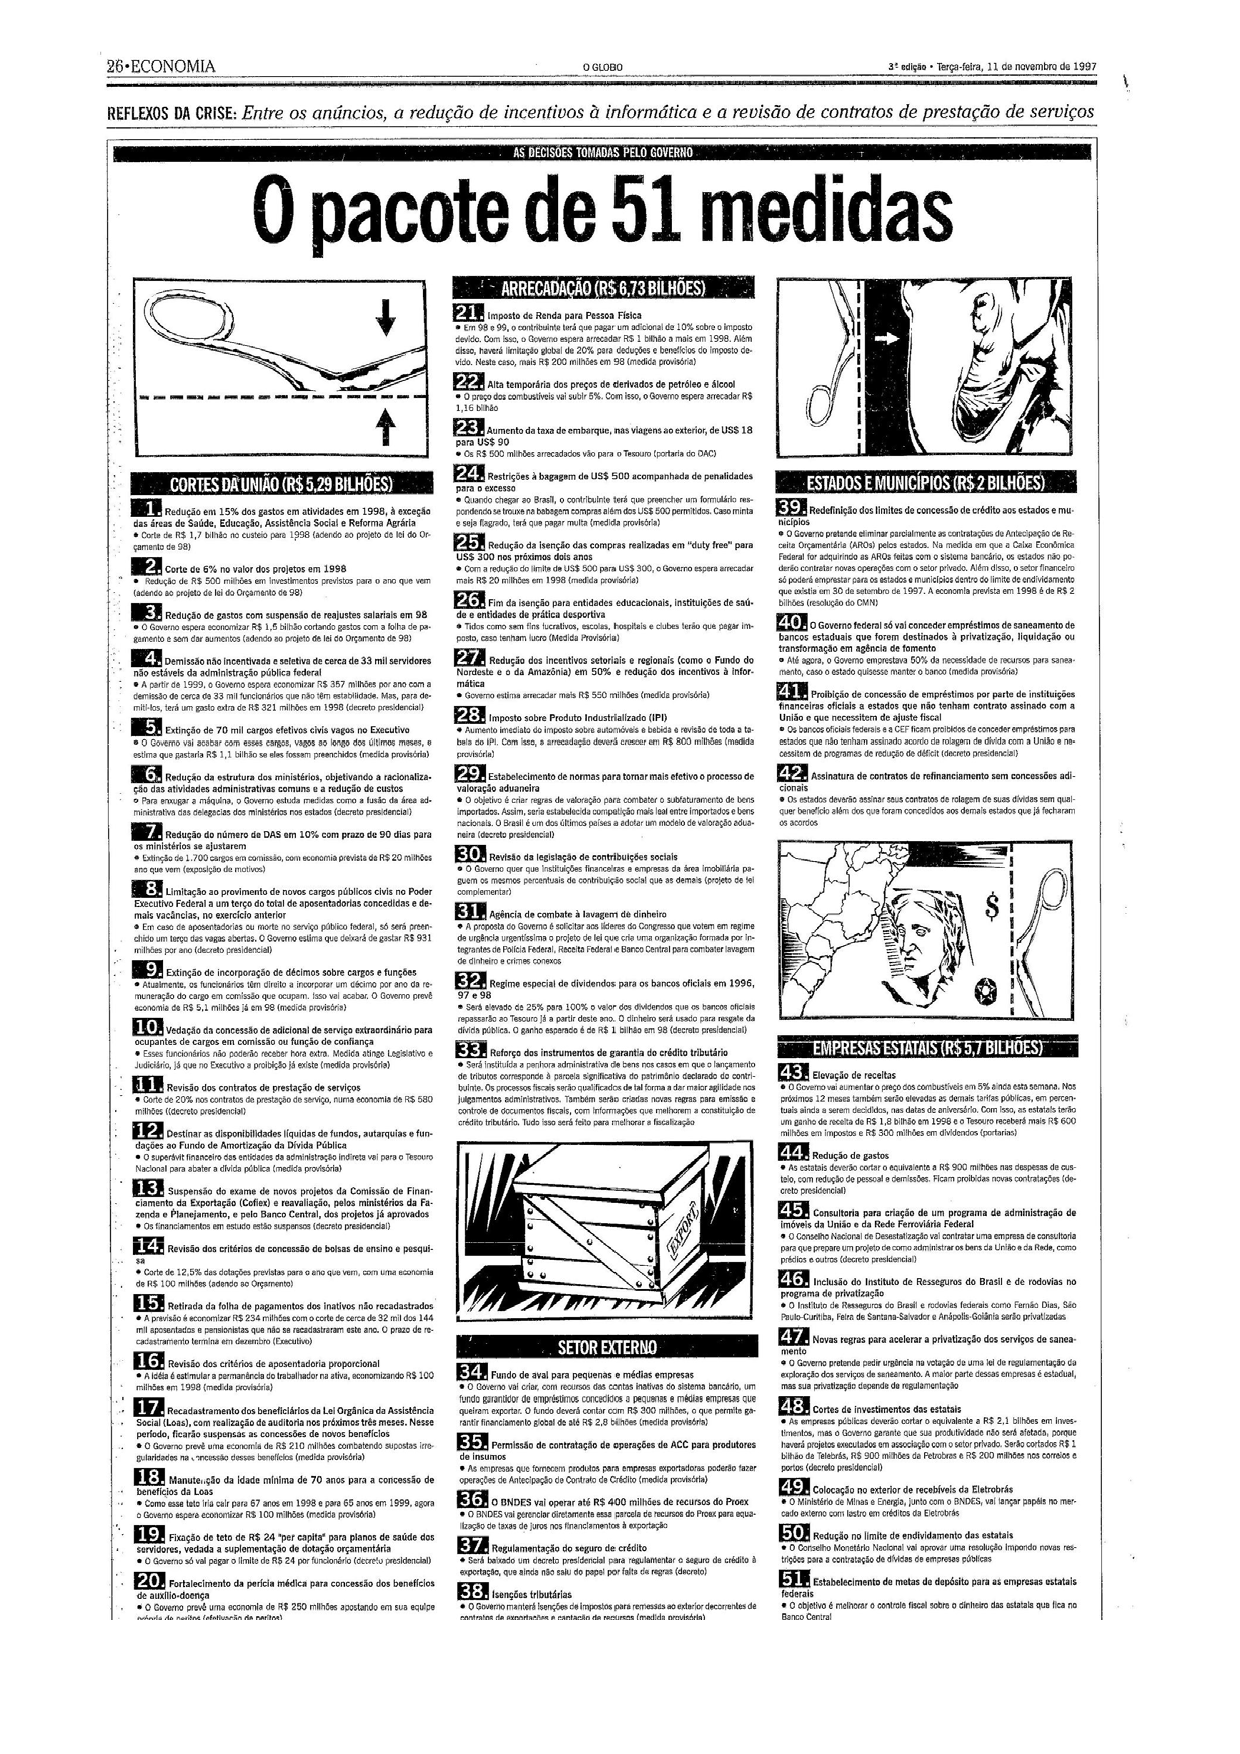
\includepdf[pages={1}]{as51medidasedit} 

O pacote teria de ser negociado: no dia 12 de Novembro, a capa do O Globo anunciava que o Congresso sugeria um aumento da CPMF ao invés de um aumento no imposto de renda. A equipe econômica, afirmava o jornal, só aceitava o aumento da CPMF se a arrecadação fosse desvinculada da saúde. Afinal, não fosse assim, o aumento da CPMF não ajudaria a reduzir o déficit. 

Mas o presidente não aceitou a mudança e o pacote sofreria resistência no congresso. Informava O Globo do dia 13 de Novembro que a bancada do PSDB, partido do presidente, era o único a apoiar integralmente o pacote. Antônio Carlos Magalhães, presidente do Senado e - normalmente - aliado do governo declarou que ``Ele (o presidente) manda lá, aqui mandamos nós. A equipe econômica manda lá, aqui mandamos nós". Do outro lado, Pedro Parente, na época secretário-executivo do Ministério da Fazenda e futuro Ministro da Casa Civil - conhecido pela a habilidade diplomática - deixou de lado a diplomacia e disse que ``Não estamos negociando nada. O conjunto de medidas é este. É o que achamos necessário. Não distribuímos benesses".

Além do tiroteio com o Congresso, o governo rapidamente se veria envolvido em um conflito, dessa vez entre membros da equipe econômica. O ministro da Fazenda, Pedro Malan, disse a um jornal argentino que o Brasil podia fazer um acordo com o FMI. A declaração viraria capa do O Globo de 18 de novembro, com a manchete ``Malan diz que acordo com FMI teria vantagens". No dia seguinte, era a vez de Gustavo Franco ser a manchete, da Folha de São Paulo: ``Acordo com FMI fere soberania, diz Franco". O Globo do mesmo dia ainda trazia o comentário de um dirigente do Banco Central dizendo que um acordo ``seria motivo para a demissão coletiva da diretoria"   

E no meio do tiroteio e da crise econômica, o governo conseguiria algumas vitórias: a reforma administrativa foi aprovada na câmara, o que traria uma economia de R\$5 bilhões, segundo a manchete do O Globo de 20 de novembro. A capa trazia ainda outra boa notícia: o Banco Central anunciava uma redução da taxa de juros, de 0,15 pontos percentuais. No dia 27 de Novembro, a capa do O Globo trazia ainda outra vitória do governo: a quebra de estabilidade do servidor foi aprovada na câmara.

No dia 29 de Novembro a Folha de São Paulo tinha como manchete ``FHC cede e muda pacote". O aumento do imposto de renda foi limitado - como ACM queria. Em compensação, o imposto sobre renda fixa cresceu. O governo também decidiu reduzir os incentivos fiscais gradualmente e desistiu de diminuir os incentivos à cultura, segundo O Globo do mesmo dia. Esse último recuo veio após diversos cineastas, diretores de teatro, atores, artistas plásticos e coreógrafos realizarem um lobby no congresso contra os cortes de gastos na parte cultural, mobilização que ocuparia duas páginas do Segundo Caderno do O Globo de 16 de Novembro. 

Dezembro seria mais calmo do que Novembro e Outubro: a crise internacional não seria capa do O Globo, e capa da Folha apenas 3 vezes, quando a crise atingiu a Coréia. Entretanto, as negociações entre empregados e empregadores para reduzir salários e as jornadas de trabalho seriam manchete várias vezes em ambos os jornais. As negociações, que começaram no setor de auto peças e rapidamente se espalharam, visavam evitar mais demissões.

Em relação a política econômica, apenas duas manchetes merecem destaque: um da Folha de São Paulo do dia 17 de Dezembro e a outro do dia seguinte, no O Globo. A Folha anunciava  ``Governo amplia seguro-desemprego". O governo decidiu aumentar o número de parcelas pagas pelo seguro desemprego e, segundo o jornal, atingiria 335 mil trabalhadores. Mas a medida custaria R\$68,23 milhões. Não deixa de ser curioso que, um mês após anunciar um pacote para reduzir gastos, o governo já tenha decidido criar novos gastos.

A manchete do O Globo não tratava sobre gastos, mas sim sobre juros: informava a noticia que ``O governo tinha a intenção de realizar uma redução brusca nos juros, devido ao agravamento do desemprego no país, mas o Banco Central so permitiu ontem uma queda mais gradual". Não demorou para que o ajuste econômico, extremamente impopular, começasse a incomodar os políticos.

Mesmo assim, os jornais trariam boas notícias - inclusive para o governo - no fim do ano, e uma certa dose de otimismo: ``Privatizações vão aliviar crise em 98" era a manchete do O Globo de 21 de Dezembro; ``Inflação de 97 foi apenas 4,4\%", informava o mesmo jornal no dia 23 de Dezembro; ``Crise não abala favoritismo de FHC", informava a Folha de São Paulo no dia 28. E fechando o ano com um golpe de ironia, no dia 31 de Dezembro a Folha trazia na primeira página: ``Bolsa lidera aplicações em 97". Mesmo com a crise, seria o investimento mais lucrativo do ano.               

\subsection*{1998}
\addcontentsline{toc}{subsection}{1998}

O ano de 1998 foi o ano de eleições para presidente, a primeira desde a redemocratização a permitir a reeleição. Também foi o ano em que a crise saiu da Ásia e se alastrou por todo o mundo, especialmente a Rússia. E o Brasil não ficaria imune, apesar das reformas que o governo pretendia executar. 

A crise mundial recomeçou logo no inicio do ano: no dia 13 de Janeiro, a manchete do O Globo era ``Banco quebra em Hong Kong e abala bolsa no mundo." Trazia ainda, no subtitulo, a informação que o governo brasileiro não reduziria os juros enquanto durasse a crise. A Folha de São Paulo era ainda mais veemente, e no mesmo dia tinha como manchete ``Crise asiática adia queda dos juros". Segundo O Globo, ``[..]cautela é a palavra de ordem do presidente e da equipe econômica. FH, dizia o mesmo jornal, garantia que não iria implementar novas medidas e que iria ``apostar todas as fichas na aprovação das reformas administrativas e previdenciárias[...]" Na mesma página, novos elogios a equipe econômica, desta vez vindo do economista Albert Fishlow. Ele afirmou que a política econômica brasileira era ``a mais realista do mundo". Outros analistas também diziam que um ataque especulativo contra o país era improvável.     

No dia 28 de Janeiro, O Globo comentava sobre o Fórum Econômico Mundial em Davos. Era a primeira vez que um chefe de estado brasileiro iria participar do evento, e a pedido dos participantes foi organizado uma sessão sobre o Brasil. O jornal também trazia uma nota com o título ``Fundos querem ouvir FH para decidir investimentos". Na nota, ficava claro que investidores tinham dúvidas sobre o Brasil. Mas grandes bancos estavam ``confiantes nas medidas que o Governo tomou para corrigir distorções e proteger o país dos efeitos da crise asiática." No mesmo dia, o caderno de economia do O Globo informava que a Indonésia tinha declarado moratória, após longos sete meses de crise. 

Se no dia 13 de Janeiro a palavra era cautela, no dia 29 a cautela foi deixada de lado: O Globo e a Folha anunciavam que os juros caíram mais do que o esperado: uma queda de 3,5 p.p. Um economista entrevistado pelo O Globo disse que ``a queda mostra que a crise no Sudeste da Ásia é um fato que já não preocupa tanto a equipe econômica. Por outro lado, o Governo está preocupado em controlar as contas públicas." Fernando Henrique, em Davos, disse que por ele, os juros ``já tinham caído ontem." E continuou: "A maior vítima dessas taxas de juros é o Governo federal[...]"

E o governo sofria com a alta de juros, e a manchete da Folha de São Paulo do dia 31 de Janeiro deixava claro: ``Gasto com juro da dívida cresce 41\%". ``A alta" informava o jornal ``é resultado do aumento das taxas de juros promovido pelo governo em outubro, para contornar os efeitos da crise asiática." Segundo os cálculos da Folha, o aumento dos juros fez com que as despesas dos Estados e Municípios aumentasse 69,32\% e as despesas do Governo federal aumentassem 28,3\%. Reduzir os juros era essencial para reduzir os gastos do governo, em todos os níveis.

Ainda em Davos, o Presidente Fernando Henrique Cardoso conversou com empresários. A reportagem do O Globo do dia 29 de Janeiro tinha como titulo ``Entre suíços, FH dá a sua reeleição como garantida. " O presidente, segundo o jornal, tranquilizou ``investidores preocupados com mudança de Governo e da política econômica" e relembrou que ``as reformas estão progredindo" e que ``até março tudo estará aprovado."

E o presidente parecia estar certo: o Senado aprovou a quebra de estabilidade do servidor, o que seria capa do dia 11 de Fevereiro tanto na Folha quanto no O Globo; e no dia seguinte ambos os jornais relatariam na primeira página a aprovação das mudanças nas regras da previdência. O objetivo era cortar gastos, evidentemente. O Globo, citando contas feitas pelo governo, afirmava que a quebra da estabilidade permitiria uma economia de R\$ 10 bilhões.                     

A alegria durou pouco: o anúncio do resultado das contas públicas de 1997 mostrou que o Governo ainda tinha muito o que fazer quando se tratava das contas públicas. No dia 27 de Fevereiro, O Globo trazia uma nota na primeira página intitulada ``Déficit é bem maior do que o esperado". A nota adiantava: o resultado do ano anterior tinha sido ``o pior dos últimos anos, superando até mesmo as expectativas dos mais pessimistas." Com déficit primário de 0,67\% do PIB, o governo gastou R\$ bilhões a mais do que arrecadou - muito distante do objetivo do governo, que era ter um superavit de 1,5\%. A Folha de São Paulo dedicou a manchete ao tema - a manchete do O Globo era sobre Sérgio Naya, dono da construtora do Palace II que tinha desabado no mesmo mês - e deixava claro: ``Dívida pública dobra no período FHC." A Folha reproduziu a declaração do porta voz do Governo, que afirmava que ``a economia ainda será beneficiada pelo pacote fiscal lançado no final de 97."

Os primeiros dos muitos sinais de que o ano eleitoral afetaria o ajuste do governo veio no primeiro dia de Março, quando O Globo publicou uma reportagem de página inteira informando que o congresso so iria trabalhar, de fato, até Abril. O motivo, a reportagem deixava claro, era as eleições em Outubro. Por isso, um projeto importantíssimo seria deixado para 1999: a reforma tributária.

O dia 5 de março traria duas notícias dignas de atenção, e relacionadas. A Folha de São Paulo trazia na primeira página ``Desemprego é o maior em 13 anos". O caderno de economia do O Globo informava a queda nas taxas de juros, e citava o desemprego como um dos motivos que levou o Banco Central a diminuir a taxa de 34,5\% para 28\%. O próprio jornal observava que ``O Banco Central deixou de lado o tradicional conservadorismo e ousou como nunca." O cenário externo melhor e o aumento das reservas também contribuiu na decisão. Mas é válido perguntar: seria essa ousadia um reflexo da necessidade de agradar os eleitores? Independente dos motivos, a ação do Banco Central seria bastante elogiada por pessoas do mercado financeiro.

%Miriam aqui no dia 05/03

Mais uma decisão com motivos políticos surgiria no O Globo de 7 de Abril: o aumento do salário mínimo para R\$130. A influência política da decisão era clara: FHC prometeu dobrar o valor do salário mínimo até o fim do mandato. O jornal também dizia que ``[...] os aliados do Governo vão pressionar por um reajuste maior para enfrentar a oposição na campanha". Mas, como o próprio O Globo observava, isso geraria mais pressão sobre as contas públicas e aumentaria o déficit.        

E se o déficit não era pequeno e as eleições pareciam aumenta-lo ainda mais, uma surpresa sobre as contas públicas seria a manchete do O Globo e da Folha de São Paulo: dois bilhões de reais não foram contabilizados nas contas de 1997, por um erro do Tesouro Nacional. O déficit de 1997 cresceu mais, chegando a R\$54 bilhões, a 6,12\% do PIB segundo O Globo. Pior: originalmente, o Governo central tinha apresentado superávit. Com o novo gasto, ele tinha passado a ser deficitário. 

A reportagem do O Globo sobre os dois bilhões a mais também falava dos resultados de Janeiro de 1998. O Governo central teve superávit e, segundo o jornal, o motivo do resultado positivo foi o aumento da arrecadação devido as medidas do pacote fiscal.

Felizmente para o governo, os eleitores não se preocupavam tanto com o déficit público, nem com os juros altos, nem com a balança comercial deficitária. Era o que apontava uma pesquisa da Vox Populi publicada no O Globo de 20 de Abril. O desemprego preocupava o brasileiro, mas os analistas achavam que isso não iria ``afetar a decisão de voto do eleitor" de acordo com a notícia. % %Fazia sentido, então, se preocupar menos com o equilíbrio das contas públicas e mais com reduzir o desemprego para atrair eleitores% %    

A principal notícia  dos jornais do dia era outra: a morte de Sérgio Motta, ministro das comunicações, amigo do presidente, mas acima de tudo, um importante articulador político do governo. Em uma das várias reportagens sobre o ministro, O Globo deixou claro que ele era o ``coordenador político do governo." Perder este importante personagem seria um golpe para o governo, especialmente para avançar com as reformas.

O golpe seria duplo, porque dois dias depois os noticiários estavam tomados pela morte de Luís Eduardo Magalhães, deputado filho de Antônio Carlos Magalhães. O Globo chamou-o de ``Um dos articuladores mais importantes do Congresso". Em menos de 48h, o governo perdeu dois homens importantíssimos para as reformas que eram tão necessárias para a economia. É difícil acreditar que a perda destes dois articuladores não tenha dificultado a vida do governo para aprovar reformas que já enfrentavam enorme resistência.

Os reflexos seriam claros: Miriam Leitão, na coluna \textit{Panorama Econômico} do dia 23 de Abril, afirmava que, com a morte de Luís Carlos Magalhães ``O Brasil ficou mais incerto, com um cenário mais turvo. Alguns líderes quando morrem levam parte da História. Ele levou parte do futuro." A coluna ainda relatava a ``estupefação do mercado financeiro" com a morte. As dúvidas sobre o futuro das reformas também ecoavam no mercado.     
   
No mesmo dia\footnote{O Globo do dia 23 de Abril circulou em duas edições. As citações da coluna \textit{Panorama Econômico} foram retiradas da segunda edição, enquanto as afirmações deste parágrafo foram retiradas da terceira edição. Ambas acessadas no acervo do O Globo.}, O Globo relatava que o governo não sabia como substituir os dois articuladores, especialmente Luís Carlos Magalhães. Na mesma página, uma nota atribuía a queda de 2,7\% da Bolsa de São Paulo a morte de Luís Carlos Magalhães. Mas a própria nota afirmava que ``[...] o mercado não espera contratempos reais tão graves para o Governo em decorrência da perda de seu líder na Câmara" 

Luís Carlos Magalhães deixou uma tarefa em aberto: a votação da reforma da previdência. Os analistas entrevistados pelo O Globo acreditavam que, se FHC assumisse a tarefa, a reforma seria aprovada sem mudanças. Não foi o que aconteceu: no dia 7 de Maio, a manchete do O Globo anunciava que a idade da aposentadoria não ia mudar. O governo tinha perdido por um voto - uma abstenção do ex-ministro do Planejamento e deputado Antônio Kandir. Uma semana depois, entretanto, o Governo conseguiria aprovar uma emenda para mudar a idade de aposentadoria de quem já estava no mercado de trabalho. Esta mudança teria efeitos imediatos sobre o caixa do governo. A economia, apenas naquele ano, era de R\$600 milhões segundo O Globo. 

Depois das tragédias nacionais, a crise internacional voltaria a ganhar destaque nos jornais. No dia 19 de Maio, tanto a Folha quanto O Globo traziam na primeira página notícias sobre a Crise na Rússia e os reflexos óbvios da crise sobre o Brasil. A Rússia, assim como o Brasil, tinha um câmbio fixo e dependia de recursos externos para financiar o déficit público. A queda na bolsa da Rússia, o aumento de juros no país e o temor que os russos não conseguissem obter recursos para financiar a dívida externa geraram especulações com o Rublo e fez com que os investidores vendessem ativos russos. O Brasil, em uma situação parecida, sofreu o impacto da crise russa, mas com menos força do que na Rússia.

Apesar da crise russa, o Banco Central anunciaria no mesmo dia uma queda de juros. A aposta dos analistas consultados pelo O Globo em 20 de Maio era que a taxa de juros sairia de 23,25\% para um valor entre 22,5\% a 22,75\%. O Banco Central reduziu a taxa para 21,75\%.  

A matéria do O Globo do dia 21 de Maio dizia que os motivos por trás do ajuste era o peso da taxa de juros na divida pública, e o desemprego crescente. Na mesma página, o jornal anunciava que o governo já tinha previsto um déficit nominal de 7,1\% do PIB em Junho. A equipe econômica esperava que o resultado do ano fosse o pior desde o início do Plano Real, com um déficit nominal de 7\%. A própria reportagem dizia que ``O pacote fiscal adotado em novembro passado foi insuficiente para compensar o aumento das taxas e os gastos adicionais do Governo." Entre estes gastos, estava o aumento do salário mínimo, que tinha sido maior que a inflação. A reportagem não trazia nenhuma declaração da equipe econômica ou de algum membro do governo dizendo se o governo iria tomar alguma atitude ou não para reduzir o déficit.

A mesma página trazia uma nota que ainda havia pressões para aumentar os gastos na área social. O próprio jornal citava que a proximidade das eleições era um dos motivos que contribuía para o aumento de gastos.   

Mesmo evitando tomar medidas impopulares, a campanha de Fernando Henrique sofreria um baque com as pesquisas de intenção de voto do fim de maio. A capa da Folha de São Paulo era ``Lula sobe e encosta em FHC". Segundo a pesquisa do Datafolha publicada no O Globo de 31 de maio, Fernando Henrique tinha 41\% das intenções de voto, e caiu para 34\%; Lula, o principal adversário, tinha 24\% e subiu para 30\%. Um dos comandantes da campanha da reeleição culpava o desemprego alto pela redução das intenções de voto.        

E o desemprego preocupava. Ele não era apenas alto, mas estava aumentando, conforme anunciava uma reportagem do O Globo do dia 22 de maio. A taxa de desemprego na Grande São Paulo chegou a 18,9\%, batendo o quarto recorde consecutivo. O aumento da População Economicamente Ativa foi um dos fatores que aumentou a taxa de desemprego, mas esse aumento também não trazia boas notícias: especialistas alegavam que parte do aumento da PEA se devia a migração para São Paulo de nordestinos afetados pela seca. 

Mas no mesmo dia da publicação da reportagem com as intenções de voto, O Globo trazia a notícia de que o governo pretendia realizar novas medidas fiscais, até junho. O subtítulo informava que ``Governo quer obter superávit primário nas contas públicas mas sem prejudicar a área social." A ideia era realizar o ajuste fiscal sem aumentar impostos, e assim recuperar a confiança do investidor internacional. O próprio jornal afirmava que ``O governo está preocupado em demonstrar ao mercado que não ficará parado assistindo ao crescimento do déficit público. Nem está imobilizado por causa da proximidade das eleições presidenciais." 

A capa da Folha de São Paulo do dia primeiro de junho seria dedicada a economia. A manchete anunciava que em março, o déficit tinha sido menor: apenas 0,78\% do PIB comparado com os quase 1\% de fevereiro. Na mesma página, uma notícia  tinha como título ``Pacote foi ruim para a imagem, diz FHC." Parece incrível que Pedro Malan tivesse anunciado no dia anterior que iria tomar novas medidas fiscais, mesmo com o Presidente admitindo que o último pacote tinha diminuído a popularidade dele. No mesmo dia O Globo informava que os aliados de Fernando Henrique Cardoso apostavam na melhora da economia no segundo semestre. 

E no dia 3 de Junho, a Folha de São Paulo trazia na capa a noticia de que o desemprego tinha recuado de 8,18\% para 7,94\%, segundo informações do IBGE. A melhora que os aliados de FHC esperavam parecia estar chegando.    

A equipe econômica anunciaria novos planos para conter os gastos. Dessa vez, o objetivo era reduzir os gastos dos estados, segundo reportagem do O Globo de 9 de Junho. O objetivo era reduzir o endividamento dos estados e aumentar o controle dos gastos públicos. Na mesma reportagem, porém, um revés para a equipe econômica: R\$ 2 bilhões obtidos nas privatizações foram destinado para a área social, ao invés de serem usados para reduzir a dívida pública, como o Ministério da Fazenda queria. E a CPMF continuava vinculada a saúde.

E apesar de ter decidido reduzir os gastos dos governos subnacionais, o governo federal anunciou medidas que aumentaram os gastos. Um dos aumentos viria por ordem da justiça: o governo foi obrigado a dar um aumento médio de 12\% aos servidores, custando R\$1,2 bilhões por ano aos cofres do Governo, segundo estimativas do O Globo de 18 de Julho. %ainda falta mais coisa nesse parágrafo

Somando-se a esse gasto, a manchete da Folha de São Paulo do dia 26 de junho era ``FHC libera gastos de ministérios." O próprio Presidente afirmava que o pacote fiscal teve ``maldades desnecessárias" e o jornal observava que ``A decisão coincide com o início da campanha eleitoral", mostrando que pelo menos o jornal acreditava em uma motivação eleitoreira para a decisão.  

O Globo do dia 10 de Julho trazia na capa que o governo ainda reduziria o Imposto sobre Operações Financeiras (IOF), para tentar aquecer a economia. A Folha de São Paulo também tinha a redução do IOF como manchete do jornal, e na capa o jornal deixava claro que o governo tinha dito que a medida não intenção eleitoral. A Folha também informava que a arrecadação do resto diminuiria em R\$763 milhões de reais, dificultando ainda mais o esforço de superávit do governo.  

%Falar do recorde externo?

Agosto seria o mês em que a crise voltaria para o Brasil. A crise russa não chegou nem perto do fim: piorou em Agosto. A Ásia ainda sofria com os efeitos da crise de 1997; e os Estados Unidos também seriam afetados pela crise global.

A Bolsa de Nova Iorque teria a terceira maior queda da história no dia 4 de Agosto e foi a manchete da Folha de São Paulo - e ganhou um espaço na primeira página do O Globo - do dia cinco. A Folha citava as incertezas na Ásia como um dos principais motivos. A queda em Nova Iorque derrubaria a bolsa de São Paulo.   

No dia 18 de Agosto, O Globo e a Folha de São Paulo dedicaram algum espaço na primeira página a moratória russa e desvalorização do rublo. No caderno de economia, O Globo trazia tanto declarações de Pedro Malan, que afirmou que ``[...]é ingenuidade ou má fé comparar a Rússia ao Brasil", quanto uma nota comparando a Rússia com o Brasil. O jornal observava que o Brasil tinha mais reservas e era politicamente mais estável, porém tinha um déficit público comparável ao déficit russo: 7,5\% do PIB no caso da Rússia, contra 7,1\% do PIB no caso do Brasil. 

Pedro Malan foi contundente ao defender que o Brasil não era bola da vez. A Folha de São Paulo citou o ministro, que disse que ``Não há razão para que a crise na Rússia tenha efeitos sobre o Brasil." Posição muito diferente era a de Maria da Conceição Tavares, que disse que se o governo mostrasse pânico, a crise viria para o Brasil. E por mostrar pânico, ela queria dizer aumentar juros: ``Se o Brasil aumentar de novo a taxa de juros, como fez na crise da Ásia no ano passado, vai mostrar pânico e passar recibo que é a bola da vez" disse a economista. 

Mas na avaliação do FMI, a Rússia não era tão importante. Mais grave era o caso do Japão, que vinha sofrendo com a crise da Ásia e em 12 de Agosto virou manchete do O Globo quando a agência de planejamento econômico do país anunciou que a economia não estava enfrentando apenas uma estagnação, mas uma recessão. 
  
O Globo trazia uma matéria no dia 19 com uma declaração do presidente do Banco Central: ``Gustavo Franco garante que perder até US\$2 bilhões de reservas não é problema." Na mesma matéria, Pedro Malan garantia que o déficit público iria fechar o ano abaixo dos 7\%. No dia seguinte, outro anúncio de Gustavo Franco: o país poderia perder até US\$ 10 bilhões sem problemas, segundo reportagem do O Globo.  

A manchete da Folha do dia 20 de agosto trazia um anúncio do ministro da Fazenda: a promessa de um novo plano fiscal após a eleição - caso Fernando Henrique fosse reeleito. Pedro Malan prometia um programa de medidas com o objetivo de gerar superávits primários e estabilizar a relação entre dívida pública e PIB. Desta vez, ao invés de apostar em um pacote, o ministro anunciava um programa de longa duração, que só terminaria em 2001.

Mas promessas não seriam o bastante: no dia 21 de Agosto, a primeira página da Folha anunciava que ``Crise atinge a América Latina e Bovespa tem queda de 6,4\%". Os títulos da dívida externa brasileira caíram para o nível mais baixo do ano - e se aproximavam do preço praticado durante a crise da Ásia. A bola da vez era a Venezuela, que também sofria com déficits fiscais, e os investidores acreditavam que iria desvalorizar a moeda. E isso tudo acontecia apesar de os japoneses anunciarem medidas para fortalecer a moeda e o mercado asiático estar se recuperando.

Não haveria trégua: no dia 22 a capa da Folha e do O Globo tratavam sobre a crise. A Folha de São Paulo dava destaque a queda na Bovespa, que levou ao acionamento do \textit{circuit breaker}. O Globo dedicou a manchete a perda de reservas internacionais: US\$2,1 bilhões ``elevando para US\$5,6 bilhões o total de perdas nas reservas internacionais em agosto." 

Mas o presidente Fernando Henrique Cardoso se mantinha confiante. ``Fernando Henrique descarta alta das taxas de juros" era o título da reportagem do O Globo, na qual o Presidente dizia que o país estava mais forte e precavido. Segundo ele, o país teve ``coragem de fazer o que era duro"

E a opinião não era exclusiva de FHC. Na mesma edição do O Globo, diversos analistas opinavam sobre a crise. Todos concordavam que a crise não era mais localizada, mas global. E muitos eram otimistas em relação ao Brasil: um economista da Confederação Nacional da Indústria (CNI) disse que ``Seria exagerado dizer que não há nada a temer, mas temos sucessos a serem contabilizados." O economista chefe do Citibank, segundo O Globo, ``acredita que o Governo brasileiro ganhou credibilidade com o lançamento do pacote fiscal no fim de 97." E isso apesar dos diversos aumentos de gastos anunciados em 1998 já tratados neste trabalho.

No domingo, dia 23 de agosto, os jornais se dedicaram a analisar os efeitos da crise. A manchete da Folha de São Paulo era sobre a perda na Bovespa: US\$83,5 bilhões no mês. O Globo trazia uma entrevista com Gustavo Franco, declarações do Presidente Fernando Henrique e a opinião de Rubens Cysne, da Fundação Getúlio Vargas.

O artigo de Cysne na página de Opinião trazia preocupações de longo prazo e de curto prazo. O economista observava que a credibilidade da política fiscal tinha sido reduzida com a ``não concretização da redução de despesas anunciada em outubro do ano passado, quando da eclosão da crise asiática e do Pacote 51[...]" Cysne ainda observava que a credibilidade é ``algo cuja perda apenas se percebe quando dela se precisa." %manter esta última frase?

Gustavo Franco, em entrevista para O Globo, tentava minimizar a crise. Segundo ele a América Latinha ``tem feito seu dever de casa." Quando questionado sobre a queda da bolsa e dos C-bonds - os títulos da dívida externa - o presidente do Banco Central disse que isto ``não são indicações da saúde do Brasil." E completou que ``A distância entre mundo financeiro e mundo real é grande." 

Ainda no caderno de economia do dia 23, Fernando Henrique garantia que o governo não lançaria um pacote fiscal naquele momento, nem nos próximos meses. E o candidato a reeleição deixaria claro: ``a prioridade ainda é o crescimento da economia, para atender às necessidades sociais do país."

No dia 24 de Agosto a principal notícia era a demissão de todo o gabinete do governo russo devido a crise econômica. Mais relevante, entretanto, era uma matéria do O Globo que dizia que o governo pretendia continuar reduzindo a taxa de juros, apesar da crise econômica. Em reunião com o presidente da república, a equipe econômica concluiu que ``o Brasil está conseguindo se diferenciar na forma como vem conduzindo as turbulências no mercado financeiro." Dado os efeitos na Venezuela e na Rússia, ``se diferenciar" significava - muito provavelmente - ir bem.

O governo tomaria medidas para aumentar as reservas, apesar de não aumentar os juros. No dia 25 de Agosto, a capa do O Globo anunciava que o Banco Central tinha tomado medidas para facilitar a entrada de dólares. Três dias depois, enquanto a manchete da Folha de São Paulo era ``Bolsas desabam no mundo", a capa do O Globo anunciava novas medidas tomadas pelo governo para atrair o capital estrangeiro. A principal medida era um corte no Imposto de Renda dos fundos externos, que ficaram isentos do IR até março de 1999. A medida foi anunciada um dia depois dos C-Bonds fecharem no menor nível histórico.          

A edição do O Globo do dia 30 de agosto dedicou dez páginas a análise da crise, com opinião dos economistas da oposição, analistas do Citibank afirmando que o país precisava aumentar os juros e uma entrevista com Pedro Malan. Na entrevista, o ministro diria que 1998 estava ``praticamente definido" e que o país cresceria 2\%. Quando questionado sobre o déficit fiscal, Malan disse que ``Nós sempre dissemos que o déficit fiscal é o grande desafio a enfrentar." Pedro Malan ainda afirmaria que o governo estava trabalhando em um programa para reduzir o déficit e que o problema era também de estados e municípios.

No dia seguinte, O Globo e a Folha reproduziam a declaração de Fernando Henrique de que não ia mudar os juros nem desvalorizar o real. No mesmo dia O Globo trazia a noticia de que o gasto da União era ``o grande vilão do déficit": o déficit do governo central era maior do que o dos governos estaduais e municipais. As despesas do governo central entre janeiro e maio tinham crescido 19\% em comparação com o mesmo período do ano anterior.

A crise continuaria em setembro. No primeiro dia do mês, a capa do O Globo e da Folha de São Paulo traziam a noticia de que a bolsa de Nova Iorque caiu 6,3\%, levando a Bovespa a cair também. No mesmo dia, O Globo trazia noticias sobre o orçamento de 1999, que tinha sido encaminhado no dia anterior para o congresso. O orçamento trazia um aumento de gastos na área social de quase um bilhão de reais em comparação com 1998. Trazia cortes em outras áreas, apesar do jornal observar que ``O ministro [do planejamento] não explicou em que áreas o Governo pretende fazer os cortes, mas já sabe que poderá enfrentar problemas no Congresso para reduzir essas despesas que são normalmente objeto de emendas apresentadas pelos parlamentares[...]" O orçamento ainda prévia superávit, mas para atingir a arrecadação prevista no projeto o governo teria que obter a aprovação do Congresso para a prorrogação da CPMF.

No segundo dia do mês, os jornais finalmente traziam uma boa noticia: alta recorde em Wall Street. A Bovespa fechou em alta de 6,87\%. Os C-bonds subiram 12\% em um dia. Mas, Miriam Leitão observava no O Globo que ``Nada muda assim de uma hora para a outra. O ataque de otimismo que o mercado teve ontem foi tão preocupante quanto os surtos de pessimismo."

Apesar da crise, o Banco Central reduziu a taxa de juros para 19\%, anunciava O Globo no dia 3 de setembro. O Globo trazia uma justificativa para a queda na taxa de juros: diminuir o impacto da dívida pública nas contas do governo. Os analistas entrevistados pelo O Globo afirmavam que os investimentos externos sairiam do país se houvesse uma desconfiança muito grande com a situação das contas públicas do Governo. Assim, mesmo que uma redução das taxas de juros afugentassem os investidores, uma taxa de juros muito alta pioraria ainda mais a situação das contas públicas, o que também afugentaria os investidores.

No dia 4 de setembro, a manchete da Folha de São Paulo e do O Globo eram dedicadas a mesma noticia: a Moody's rebaixou a nota do Brasil, colocando o país com a mesma nota da Venezuela. A decisão seria atacada por Pedro Malan e por economistas de bancos. O economista chefe para Mercados Emergentes da Goldman Sachs chamou o rebaixamento de ``um delírio total." Malan atacaria a Moody's, alegando que o rebaixamento era apenas uma tentativa da agência de se preservar: a Moody's tinha classificado os países da Ásia que foram duramente afetados pela crise de 1997 como muito confiáveis. Mas o estrago estava feito e a Bovespa caiu 8,6\% no dia do anúncio.

A queda de 8,6\% da Bovespa seria o menor dos problemas, porque no dia seguinte ao anúncio da Moody's a bolsa chegou a cair 13,9\% mesmo após o acionamento do \textit{circuit breaker} e fecharia em baixa de 6,13\%. O efeito pior seria sobre as reservas: o país perderia US\$2,59 bilhões em um dia e o Banco Central se viu obrigado a subir as taxas de juros para 29,75\%.

Depois do aumento dos juros, a capa da Folha de São Paulo do dia 6 de Setembro trazia uma frase sobre a crise de um dos membros do Conselho Editorial: ``A perda de confiança tornou inevitável ao governo dar um sinal de vida." O governo daria.

O Globo do mesmo dia trazia uma reportagem afirmando que o governo iria adotar mais medidas para reduzir o déficit público. O jornal dizia que o objetivo do governo era reduzir o déficit público de 7\% para 3,5\% até 2001, e não aumentar o déficit nominal em 1998 - apesar do aumento de juros. Isso só poderia ser realizado com cortes no gastos ou um aumento na arrecadação ou com uma combinação dos dois. O jornal garantia que haveriam cortes de gastos. 

Apesar da crise, a Folha de São Paulo trazia na capa uma notícia boa para o governo, especialmente para FH: em pesquisa feita pelo Datafolha, 54\% dos eleitores consideravam Fernando Henrique mais bem preparado para enfrentar a crise, contra 16\% que tinha a mesma opinião em relação ao candidato da oposição. 

No dia 8 de Setembro, a capa do O Globo anunciava que o governo deveria apresentar no mesmo dia propostas para cortar gastos. Muitos ministros protestaram contra a ideia, dizendo que não tinham mais nada para cortar. Um ministro afirmou que podia ``cortar um pedaço do braço" dele. Não importava: ``a decisão do presidente é de defender a moeda, mesmo que isto signifique adotar medidas impopulares" dizia Míriam Leitão em sua coluna no jornal no mesmo dia do anúncio. A coluna \textit{Panorama Econômico} trazia informações de que o governo estaria planejamento um mecanismo novo de controle de gastos e que haveria cortes nas pastas de Comunicações e Transportes. E a coluna informava que o governo não pretendia fazer nada contra o mercado: não quebraria as regras, não criaria proibições, não centralizaria o câmbio. O objetivo era ``conquistar a credibilidade e convencer o investidor a ficar porque é um negócio lucrativo." Para um país que tinha vivido confiscos, congelamento de preços e outros experimentos na política econômica, essas eram boas notícias.

No dia seguinte, O Globo publicaria uma matéria sobre o pacote fiscal anunciado no dia anterior. As novas medidas - que não receberam o nome de pacote porque o governo temia amedrontar os eleitores - cortava, imediatamente, R\$4 bilhões em gastos. Ficavam indisponíveis 20\% dos recursos que seriam repassados para investimentos e custeio em 1999, o equivalente a R\$8,6 bilhões. E um número muito próximo foi estabelecido como superávit do ano seguinte: R\$8,7 bilhões. O governo se comprometia em enviar para o congresso até 15 de novembro um ``programa de ajuste fiscal com metas de redução do déficit público entre 1999 e 2001" segundo O Globo.

O que aconteceu com o Pacote 51, anunciado em novembro de 97? Essa era uma pergunta feita e respondida na edição do O Globo de 9 de Setembro. O governo foi obrigado a recuar de muitas: a demissão de 33 mil servidores não estáveis foi adiada devido a alta do desemprego; o aumento do IPI sobre automóveis foi revogado devido a queda nas vendas; o fim da isenção de impostos para entidades educacionais e instituições de saúde foi alvo de uma briga na justiça que o governo perdeu.   

A Folha de São Paulo e O Globo dariam enfoques diferentes ao pacote: O Globo trazia na manchete a notícia de que a saída de de dólares tinha sido contida. A Folha de São Paulo era muito mais crítica e tinha como manchete ``Medidas fiscais não convencem o mercado." A Bolsa de São Paulo, informava a Folha, operava em alta de 5\% até o anúncio do pacote, e fechou em queda de 0,34\% - na contramão da Bolsa de Nova Iorque. 

As medidas fiscais realmente não convenceram, como ficou claro nos dias subsequentes ao anúncio. A Folha de São Paulo do dia 10 trazia, na capa, que ``Cerca de US\$2 bilhões deixaram o país nos dois primeiros dias após a alta dos juros e o anúncio de medidas fiscais." Tanto O Globo e a Folha ressaltavam que o Banco Central tentou leiloar papeis pré-fixados - com os juros a 28\% - os bancos não compraram. Segundo O Globo do mesmo dia, as taxa de juros que os bancos pediam eram entre 34\% e 50\%. Francisco Lopes, diretor do Banco Central, anunciou que não haveria um aumento grande da taxa de juros. 

O Banco Central desistiria de manter os juros no nível que estavam. Ao contrário do que Francisco Lopes tinha prometido, a taxa de juros aumentou 20\% e foi para 49,75\% no dia 10. O anúncio do Banco Central ocorreu depois de FHC descartar outra elevação na taxa de juros, informava a Folha de São Paulo do dia 11 de Setembro. O mesmo jornal trazia a informação que o presidente tinha declarado que o governo ``chegou ao limite máximo" do corte de gastos.       

E mesmo os cortes de gastos e o aumento de juros não afetariam o favoritismo de Fernando Henrique para a reeleição. No mesmo dia em que os jornais anunciavam o aumento de juros, O Globo trazia uma reportagem com uma pesquisa de intenções de voto realizada pelo Ibope que mostrava que o presidente tinha subido 3\% nas pesquisa e agora tinha 47\% das intenções de votos.              

No dia 12 de setembro, os jornais traziam o resultado das ações do governo: a Folha de São Paulo tinha como manchete ``Bolsa reage, mas dólar continua a sair". O Globo trazia manchete parecida, mas trazia a informação do Banco Central de que a saída de US\$ 1,7 bilhões era de operações realizadas antes do aumento de juros. A bolsa subiu 13\%, ajudada pelas compras realizadas pelo BNDES e pelo anúncio que o FMI estava disposto a ajudar o país. Os C-bonds também voltaram a subir. Mesmo o mercado de câmbio ficou mais estável, informava O Globo, e a cotação do dólar futuro, segundo o jornal, teve ``queda forte". Um possível suporte do FMI tranquilizou os mercados, embora Stanley Fischer - na época vice-diretor-gerente do FMI - tivesse deixado claro que o Brasil não tinha pedido assistência financeira.

Apesar do suporte do FMI, a Folha de São Paulo do dia 12 de setembro contava com uma reportagem intitulada ``Analistas veem Brasil como foce de crise." Segundo 14 dos principais analistas da América Latina, o Brasil tinha ``problemas estruturais urgentes, que se não forem solucionados com uma combinação de reforma fiscal severa anunciada pelo governo imediatamente e ajuda financeira externa, podem colocar em risco o real" - uma análise bem diferente daquela de 1997. Os analistas deixavam claro que o governo precisava agir, e um deles afirmava que ``Se o temor do presidente é a eleição, não acredito que a tomada de medidas fiscais, mesmo impopulares, vão fazê-lo perder. Pelo contrário, os eleitores vão entender isso." 

Os efeitos do aumento de juros sobre as contas públicas também foi notícia. O Globo informava que o ajuste podia custar R\$20 bilhões para o Governo. Na mesma matéria, o jornal afirmava que, para a maioria dos analistas, as medidas tomadas pelo governo não eram o bastante. Era necessário um ``ajuste fiscal mais duro para que o país recobre sua credibilidade". 

Com o país sofrendo com uma imensa crise econômica e a vinte dois dias das eleições, é evidente que o clima se acirrava. Em 26 de agosto de 1998, ainda no começo da crise, O Globo trazia uma matéria com o título ``Oposição pede a demissão da equipe econômica". E no dia 12 de setembro, O Globo trazia uma declaração, desta vez vinda da base aliada: ``ACM culpa Congresso por turbulência", era o titulo. Para Antônio Carlos Magalhães, o fato do Congresso não ter aprovado as reformas tinha deixado o país vulnerável a crise. E, para o senador, a oposição era responsável pelo fato das reformas não terem sido aprovadas.   

O jornal trazia, na mesma página, uma nota sobre a situação das reformas. A reforma tributária, da previdência e administrativa tramitavam há três anos, segundo o jornal. A tributária sequer tinha saído da comissão que examinava; a reforma da previdência foi ``desmontada na Câmara em 1996, remontada no Senado em 1997 e novamente desfigurada na Câmara, no final do semestre passado". Vários pontos da reforma administrativa tinham sido aprovados como o governo queria, mas muitos pontos ainda precisavam ser regulamentados em lei - como a demissão de funcionários dos três níveis do governo.

E a preocupação dos políticos com a crise era tanta que a Folha de São Paulo dedicou uma página do caderno especial sobre eleições do dia 13 de setembro - bem como a capa do jornal, que era tomada por uma imensa interrogação ao invés de uma foto - para tratar sobre o ``pacto nacional" contra a crise que Fernando Henrique articulava. A ideia era obrigar o congresso a aprovar a reforma da Previdência e  de acordo com o jornal, um ``remendo da reforma tributária". O jornal já discutia se o remédio contra a crise seria ``mais amargo que o imaginado até agora".

%A proposta de Bill Clinton de ajudar a América Latina foi capa da Folha de São Paulo no dia 15, e a capa do mesmo jornal no dia seguinte informava que o anúncio reanimou os mercados. 

O remédio seria mais amargo, com O Globo do dia 17 de setembro anunciando que o governo iria realizar um corte adicional de R\$ 2 bilhões de reais. O principal corte era nos investimentos das estatais. E mais tentativas de ajustar as contas públicas seguiriam: a manchete do O Globo do 19 informava que o presidente Fernando Henrique tinha apesentado ``a primeira proposta concreta de mudança no projeto de reforma tributária". E o governo voltava a se contradizer: no dia 22, O Globo tinha como manchete ``Governo já não descarta o aumento de impostos". A própria reportagem lembrava que o governo tinha dito que não iria aumentar impostos.

No dia 24 de setembro os jornais finalmente traziam novas declarações de Fernando Henrique sobre a crise. A manchete do O Globo era enfática: ``FH diz que fará ajuste `rápido e rigoroso' e reanima mercados". A Folha de São Paulo destacava que era o primeiro discurso do presidente sobre a crise internacional. Os dois jornais concordavam que o presidente tinha deixado claro a necessidade do ajuste. O Globo falava em ``um ajuste rigoroso, rápido e definitivo" e citava o presidente: ``Precisamos fazer o Estado viver dentro de seus limites". A Folha trazia um editorial que começava com a seguinte frase: ``A dez dias da eleição, o presidente teve a coragem de reconhecer diante do país que não é mais possível adiar um doloroso acerto de contas nacionais".         

O discurso trazia poucas propostas: pedia firmeza aos brasileiros, defendia um ajuste nas contas públicas, pedia a provação das reformas paradas no congresso. Mais interessante era que Fernando Henrique não tinha falado de improviso, como normalmente fazia, mas tinha lido um discurso escrito por Gustavo Franco e revisado por Malan e André Lara Resende, um dos pais do Real e na época presidente do BNDES. Seria o discurso apenas um ``sintoma" da equipe econômica ter ganho mais espaço no governo?

O discurso seria bem recebido por instituições internacionais bem como pelo mercado. A Bovespa fecharia em alta de quase 11\%. O FMI, o BID, o Banco Mundial e o secretário do tesouro americano lançariam notas elogiando o discurso. Os três primeiros ainda ofereciam recursos para o país realizar as reformas.              

O Globo do dia 25 de Setembro trazia propostas concretas. A ideia era criar um gatilho que cortasse alguns gastos automaticamente toda vez que o déficit público atingisse um valor específico. A reportagem também trazia o porta voz do governo dizendo que ``A posição do presidente também é a de preferir que os impostos não sejam aumentados". Não que essa fosse a principal notícia: a primeira página do O Globo dava mais importância a quebra do LTCM, fundo administrado por dois nobéis de economia. Na Folha de São Paulo, a manchete era a possibilidade de um aumento da CPMF.

%dia 26?

E além dos mecanismos para cortar gastos no nível federal, era necessário o apoio dos estados. E a grande maioria dos favoritos nas eleições para governador aceitavam fazer um pacto contra crise com FHC, se ele fosse reeleito no primeiro turno, informava O Globo no dia 27. Até membros de partidos da oposição, como PT e PDT, apoiavam o pacto. E a primeira página da Folha do mesmo dia anunciava que as medidas de ajuste não tinham afetado as intenções de votos de Fernando Henrique, que continuava sendo o favorito.

O ajuste fiscal seria importantíssimo para o acordo que o governo estava fazendo com o FMI. Seria necessário dobrar o superávit primário de 1999, informava a capa do O Globo de 28 de setembro, para fechar um acordo com o Fundo. O ministro da Fazenda viajou no dia 29 para negociar com o FMI o ajuste necessário para receber a ajuda.

No último dia de setembro, o tamanho da ajuda já começava a ser discutido: O Globo falava em mais de US\$ 30 bilhões disponibilizados pelo FMI. A ideia não era que o país iria usar todos os recursos disponíveis, mas ``causar impacto psicológico nos mercados financeiros" de acordo com um alto funcionário do Governo americano. 

O Presidente do Banco Central, Gustavo Franco, que em 1997 tinha sido contra um acordo com o FMI, era favor do acordo desta fez, segundo O Globo do mesmo dia. E, mais uma vez, Gustavo Franco deixou claro que estava descartada uma mudança da política cambial.

A Folha de São Paulo trazia, no dia 2 de outubro, a manchete com o tamanho do ajuste que o FMI queria que fosse feito nas contas públicas: US\$25 bilhões, 3\% do PIB. O jornal ainda informava que ``Cerca de dois terços desse valor podem vir de cortes de gastos, especialmente dos Estados, e por meio de reformas. O resto, provavelmente, terá de ser obtido com aumento de imposto." 

E depois de várias declarações otimistas, a Folha traia uma declaração bastante pessimista. Dessa vez, a declaração vinha de Rudiger Dornbusch, do MIT, que previu uma desvalorização do real ``em até três meses e profunda recessão no Brasil em 1999". Para evitar a catástrofe, Dornbusch sugeria um ajuste fiscal e controle do câmbio. 

No dia seguinte, era a vez do O Globo relatar o pacote. O ajuste que o jornal relatava era menor do que o anunciado na Folha de São Paulo: US\$ 20 bilhões. A coluna de Míriam Leitão no jornal adiantava que, se reeleito, Fernando Henrique faria um ``pronunciamento à Nação explicando o sentido do ajuste fiscal. Não será anunciado pacote, mas uma direção. As medidas serão detalhadas depois." Do lado da coluna, uma reportagem informava que o Governo não iria aplicar nenhum ``pacote econômico bombástico". O principal medo era uma desvalorização súbita.

O que o Governo começava a executar era um corte de gastos. Informava a coluna \textit{Panorama Econômico} que o governo já tinha preparado a regulamentação da reforma administrativa. A redução das despesas seria de R\$ 7 bilhões se a regulamentação fosse aprovada.

As eleições ocorreriam no dia 4 de outubro. Já no dia 5, era anunciada a reeleição de Fernando Henrique Cardoso no primeiro turno. O resultado oficial só sairia dias depois, mas o presidente tinha pressa. No dia 6 de Outubro a manchete do O Globo era ``FH manda equipe econômica acelerar programa de ajustes". O programa não era um pacote, como das outras vezes, dizia Pedro Parente, secretário executivo da Fazenda. Era um ``plano de ação de médio prazo", com medidas ``concentradas em cortes de gastos, e todas serão submetidas ao Congresso".

Não se sabia quais medidas seriam tomadas na prática para conter o déficit. Os anúncios eram genéricos: ``O governo só vai se comprometer com o que for factível" dizia uma fonte envolvida nas negociações ouvida pela coluna Panorama Econômico. A ideia era um plano de superávits fiscais até 2001. A ajuda do FMI só sairia com o anúncio das metas.            
 
O Globo do dia 6 de Outubro também trazia declarações de Gustavo Franco. A reportagem não trazia surpresas vindas dele. O presidente do Banco Central anunciava que não haveria mudanças no ritmo da desvalorização, apesar de existirem opiniões contrárias a essa posição, inclusive dentro do próprio FMI. E também dizia que eles estavam ``trabalhando no plano fiscal, como foi determinado pelo presidente Fernando Henrique, e teremos notícias sobre isso a qualquer momento". 

Gustavo Franco também falou do Pacote 51, explicando que as medidas adotadas tinham deixado áreas do setor público fora de controle, o que impediu o ajuste. Dessa vez, ele dizia, o problema seria resolvido. E os juros cairiam rapidamente.

A primeira medida de ajuste já seria anunciada nos jornais do dia 7 de outubro: corte de 12.500 vagas no serviço público. Fernando Henrique anunciaria, segundo O Globo, mais medidas no mesmo dia. O que estava em estudo, segundo o jornal, eram mais cortes de gastos - inclusive cortes nos incentivos ficais, previstos no Pacote 51 mas nunca executados - e o mecanismo de cortes automáticos. Em relação aos impostos, estava em estudo o aumento da CPMF e do imposto de importação de petróleo e a prorrogação no aumento do imposto de renda.

O corte de gastos ganharia um aliado curioso: ACM informou ao presidente, segundo O Globo, que o Congresso não iria apoiar um aumento de impostos antes do governo cortar gastos. Mas a Folha de São Paulo trazia uma versão diferente: ACM não teria colocado nenhuma condição e teria dito que o ideal era aumentar a CPMF. 

No dia 8 de Outubro, O Globo e a Folha de São Paulo traziam informações desencontradas sobre a declaração do presidente. A Folha dizia que as medidas de cortes de gastos seriam apresentadas no dia 20. O jornal O Globo dizia que elas estariam prontas dia 20, mas só seriam anunciadas após o segundo turno das eleições porque aliados do governo estavam preocupados com os efeitos que o anúncio teria sobre o resultado do segundo turno.

Mas o discurso do presidente trazia novidades. O Globo trazia no primeiro parágrafo da primeira página o anúncio que FHC queria aprovar um imposto sobre grandes fortunas - projeto do próprio Fernando Henrique quando foi Senador. E que também aumentaria a CPMF de 0,2\% para 0,3\%. Além dessas duas propostas, o presidente dizia que o ajuste seria duro, segundo O Globo. Também convocava a oposição para o diálogo. A Folha de São Paulo dava destaque a declaração do presidente de que havia gente demais no serviço público e que ele combateria ``a ineficiência da máquina, os privilégios". O discurso não conteve a sangria de dólares, e no dia 9 de Outubro a Folha trazia uma reportagem dizendo que a quantidade de dólares que saiu em no dia anterior (8 de Outubro) tinha sido maior do que no dia 7.

 No dia seguinte a declaração do presidente, dia 9, a primeira página dos jornais falava sobre a nota conjunta divulgada pelo FMI e pelo Governo brasileiro. Tanto a Folha quanto O Globo ressaltavam que o comunicado dizia que não haveria mudanças na política cambial e nem controle de capital. Além disso, os compromissos que já vinham sendo relatados pelos dois jornais: honrar as dívidas, manter os juros flexíveis e obter um superávit primário de 3\% do PIB em 1999.

A nota conjunta foi bem recebida pelo mercado. A Bovespa, que operava em queda, fechou com uma pequena alta. Mas a nota, como observava a Folha de São Paulo, não dizia nada sobre o valor do apoio financeiro que o FMI daria ao Brasil, nem quando o acordo seria formalizado.

Não demorou muito para que a informação aparecesse. No dia 10 de Outubro, a manchete do Globo trazia o tamanho da ajuda externa que já tinha sido garantido para o Brasil: US\$ 24 bilhões, sendo US\$15 bilhões do FMI. Mas o valor poderia aumentar com a contribuição dos países do G-7. 

A bolsa voltaria a subir: a Bovespa fecharia em alta de 5,7\%. Não era a única boa notícia: a compra de um banco brasileiro por um banco estrangeiro fez com que o pais tivesse fluxo cambial positivo, segundo O Globo. A Folha de São Paulo informava que a Bolsa de São Paulo tinha subido quase 11\% desde o comunicado conjunto. 

Os economistas voltariam a ficar otimistas. José Márcio Camargo, ouvido pela coluna Panorama Econômico, achava que o comunicado conjunto tinha exorcizado os três fantasmas que ameaçavam o Brasil: a desvalorização cambial, a moratória e o controle de capitais. Ele não falava em enxurrada de dólares, mas que ``os dólares de residentes podem voltar".        
 
Novas boas noticias, desta vez vindas dos Estados Unidos. A primeira página do O Globo do dia 16 tinha como manchete ``EUA voltam a reduzir juros e dão verba extra para FMI evitar crise". Além dos recursos extras que poderiam ajudar o Brasil a Bovespa subiu 6,64\%. O Globo também informava que os técnicos do governo viajavam para Washington para apresentar as medidas do ajuste fiscal para o FMI. 

No dia 21 de Outubro, o ajuste fiscal ganharia novos contornos. Segundo O Globo, o Brasil e o Fundo Monetário Internacional tinha acertado que o ajuste em 1999 seria de 23 bilhões. O tamanho do superávit iria crescer progressivamente: 2,6\% em 1999; 2,8\% em 2001; e 3\% em 2001.         
 
A Folha de São Paulo trazia informações de como seria feita a divisão do superavit: a União ficaria com maior parte do ajuste, tendo que gerar um superavit de 1,8\% do PIB. Os 0,8\% restantes seria divididos igualmente entre estatais e governos sub-nacionais. 

E, além do aumento na CPMF e o imposto sobre grandes fortunas, O Globo discutia a proposta de um aumento na contribuição da previdência, e passar a cobrar a contribuição dos servidores inativos. E também se falava um novo imposto sobre o combustível, que geraria uma receita extra de R\$1,5 bilhão. Já em relação a redução de despesas, O Globo informava que ``Ficou decidido com o Fundo que o programa de ajustes terá como base reformas estruturais. No entanto, não chegam a ser detalhadas que reformas serão essas e quais as medidas a serem implementadas. Essa discussão ficará para a próxima etapa das negociações". 

Pedro Parente, que negociava a ajuda do FMI, deixou claro o quão crítica era a situação do país. A manchete da Folha de São Paulo trazia o que Parente tinha dito sobre o tema: ``Sem ajuste fiscal, setor público vai `falir'". O jornal ainda traia a informação que o ajuste fiscal não deveria contar com o imposto sobre grandes fortunas, e que traria medidas para atenuar os impactos do programa. A principal medida estudada para atenuar os impactos do programa era o pagamento de benefícios para aqueles que estivessem desempregados há mais de 12 meses.     

O plano de ajuda ao país cresceria: O Globo do dia 23 de Outubro informava que o Fundo Monetário Internacional tinha anunciado que a ajuda ao Brasil seria de US\$30 bilhões. Na mesma reportagem, Fernando Henrique Cardoso projetava que o país poderia obter um crescimento razoável após seis meses de ajuste. Mas a Folha de São Paulo destacava que Stanley Fischer disse que o acordo dependia do ajuste fiscal. E o ajuste estava ameaçado.

Os partidos da base aliada do governo ameaçavam, segundo O Globo, ``inviabilizar o ajuste fiscal". A raiz do conflito eram as eleições: ministros do governo e tucanos estavam apoiando candidatos da oposição no segundo turno em alguns estados. Informava a reportagem que os ministros da Saúde e Educação estavam apoiando o candidato do PT no Distrito Federal.

E a resistência não era só no congresso: no dia 27 de Outubro, um dia antes do anúncio do ajuste fiscal, a Folha de São Paulo trazia a informação de que governadores recém eleitos resistiam ao ajuste fiscal. A resistência não era só da oposição, mas vinha até mesmo de governadores do partido do presidente. O governador do Rio, Anthony Garotinho, iria na contra mão do ajuste: a Folha falava que algumas das propostas dele eram aumentar salários e contratar mais funcionários públicos. 

Mas a rebeldia da base aliada e a resistência dos governadores não impediu Fernando Henrique ir a televisão para anunciar o ajuste, que agora tinha nome: Programa de Estabilidade Fiscal. No dia 28 de Outubro, as declarações do presidente eram a capa dos jornais. O Globo destacava que FH tinha dito que ``os cortes sem precedentes vão acabar com o flagelo dos juros altos". Menos otimista, a manchete da Folha era simplesmente ``FHC anuncia carga tributária maior".

O ajuste trazia cortes e aumentos de impostos, mas também tinha o objetivo era fazer um ajuste justo, cobrando ``mais de quem pode mais. E menos de quem tem menos", nas palavras do presidente . A CPMF iria aumentar para 0,3\%; a contribuição dos servidores públicos - inclusive os inativos - para a previdência aumentaria. Mas também haveria um corte de gastos de R\$8,7 bilhões. 

Mas o presidente tinha deixado claro que somente as reformas dariam uma solução permanente para o problema. O discurso feito por FHC - reproduzido na integra pela edição do dia 28 de Outubro do O Globo - um trecho merece destaque: o presidente alegava que ``o Governo não poderia mexer em cerca de três quartos do orçamento. Isso incluía gastos com o funcionalismo e transferências para estados e municípios, e o presidente observava que estas transferências vinham ``crescendo de modo expressivo". Portanto, continuava o presidente, a única opção era cortar os gastos com saúde, educação e assistência social. Por isso a urgência das reformas, explicava Fernando Henrique. 

O discurso pedia para o congresso aprovar as medidas com urgência. Informava a Folha do dia 28 que, felizmente para FH, o PMDB tinha conseguido controlar a rebelião interna que pregava o fim da aliança com Fernando Henrique. Mas o partido queria ``discutir com o governo o pacote fiscal", segundo o jornal.             

 
 
\section{Conclusão}

Em janeiro de 1999, o governo abandonaria o câmbio fixo, contra a vontade de diversos membros da equipe econômica. A medida traria diversos problemas para a economia, que fogem do escopo do trabalho,mas a estabilização sobreviveria.

Afetado por duas graves crises internacionais entre 1996 e 1998, a indecisão do governo custou caro. É possível que a crise em 1998 não tivesse sido tão grave se em 1997 o Pacote 51 realmente tivesse sido posto em prática, ou se as reformas na constituição tivessem sido aprovadas. Porém, reformas constitucionais - especialmente aquelas que afetam a previdência e os funcionários públicos - são extremamente impopulares, assim como outros cortes de gastos. De fato, até hoje essas medidas são impopulares, como se pode ver no cenário atual.

O presidente Fernando Henrique precisaria convencer os aliados a votar a favor das reformas. O custo dessa mobilização era duplo: politicamente, as reformas podiam gerar atritos na base aliada; e ainda, as negociações poderiam envolver ``trocas" que pesariam ainda mais no orçamento. Por exemplo, os parlamentares podiam se recusar a votar as emendas até os recursos para projetos deles serem liberados, como ocorreu na votação da reforma na previdência em 1996. 

E ainda, o presidente teria de enfrentar a reação de eleitores que fossem afetados pelas medidas. E as medidas afetavam muitos eleitores. A aprovação das reformas podia custar a reeleição de FHC. %escrever mais aqui

O governo ainda sofreria com uma corrosão da credibilidade. Ao anunciar um pacote fiscal e não executar o prometido, o governo gerou desconfiança por parte dos investidores. Episódio emblemático ocorreu durante a crise em 1998, quando o governo anunciou que não aumentaria os juros no dia 10 de setembro e no dia seguinte aumentou os juros. Estas contradições reforçaram as desconfianças dos investidores. 

Mas a perda de credibilidade também tem raízes políticas: o Pacote 51 foi mutilado, em parte, por razões políticas. O aumento do Imposto de Renda, ajuste proposto no pacote, foi negociado no congresso por resistência política. Outro corte proposto no Pacote 51, a redução dos incentivos fiscais em 50\%, fracassou graças a resistência do congresso em aprovar a medida. 

E o componente eleitoral não pode ser ignorado. Alguns cortes de gastos seriam revogados logo no início da campanha eleitoral, como observado na análise de 1998. E cortar gastos afetaria o crescimento econômico. Um dos motivos das demissões previstas no Pacote 51 não terem sido executadas foi justamente o alto desemprego que afetava o país. Um aumento no desemprego, por medidas tomadas pelo governo, poderiam reduzir muito a popularidade do mesmo.

Ainda assim, é notável que em 1998 Fernando Henrique tenha tentado uma nova reforma. Mesmo antes das eleições, com o cenário econômico se deteriorando, o presidente tentava avançar com algumas reformas para melhorar a situação do país, incluindo aqui reduções de gastos. Mas no fino equilíbrio entre reformas econômicos impopulares e o projeto de reeleição, o projeto de reeleição era a prioridade.

A economia brasileira precisaria de ajustes muito mais profundos, como já observado, para a âncora cambial sobreviver. O mesmo ajuste, provavelmente, deixaria o país menos vulnerável a especulação internacional, com investidores externos mais confiantes em relação ao futuro do país. Mas todo o ajuste está, em última instância, sujeito as possibilidades políticas: sem o apoio do congresso, as mudanças são impossíveis. Se os políticos tiverem outras prioridades além da estabilidade econômica - a reeleição, por exemplo - os ajustes podem ser preteridos. Os anos de 1998 e 1999 no Brasil mostram o que acontece quando as prioridades políticas são postas acima da boa condução da política econômica.   

\begin{thebibliography}{16}
 \bibliographystyle{plainnat}

\bibitem[Franco(2005)]{Francoxxxx}
FRANCO, G.H.B.
\emph{Auge e declínio do inflacionismo no Brasil} em Fabio Giambiagi et al
\textbf{Economia brasileira contemporânea}
$1^{a}$ edição
Rio de Janeiro: Elsevier, 
2005 p.258-283 

\bibitem[Giambiagi(2002)]{Giambiagi2002}
GIAMBIAGI, F.
\emph{Do Déficit de Metas às Metas de Déficit: a política fiscal do período 1995-2002}
\textbf{PPE}, 
Abril de 2002. \\
Disponível em: $\langle$http://www.ppe.ipea.gov.br/index.php/ppe/article/viewFile/277/214$\rangle$
Acesso em 12/12/2014

\bibitem[Grossmann(1998)]{Grossmann1998}
GROSSMANN, S. P.
\textbf{Desempenho das Contas Públicas no Real: Uma análise da política fiscal no período 1993-1997}
Rio de Janeiro, 1998. Dissertação de Mestrado - Pontifícia Universidade Católica do Rio de Janeiro

\bibitem[Werneck(2014)]{Werneck2014}
WERNECK, R.L.F. \emph{Consolidação da estabilização e  reconstrução institucional, 1995-2002} em 
ABREU, M. P. (org.). 
\textbf{A Ordem do Progresso: dois séculos de política econômica no Brasil.}
2ª edição.
Rio de Janeiro: Elsevier,
2014. p. 331-356


\end{thebibliography}

\end{document}